%% ============================================================
%%  RAPPORT PFE – MASTER PROFESSIONNEL EN CYBERSÉCURITÉ
%%  SprintUp – Couche d'agents IA (RAG + MCP)
%%  Fichier principal — compiler avec pdfLaTeX + Biber
%% ============================================================
\documentclass[12pt,a4paper,oneside]{book}

%% ── Encodage & Langue ──────────────────────────────────────
\usepackage[utf8]{inputenc}
\usepackage[T1]{fontenc}
\usepackage[french,english]{babel}

%% ── Mise en page ───────────────────────────────────────────
\usepackage{geometry}
\geometry{top=2.5cm, bottom=2.5cm, left=3cm, right=2.5cm,
  headheight=15.5pt}
\addtolength{\topmargin}{-3.5pt}

%% ── Interligne ─────────────────────────────────────────────
\usepackage{setspace}
\onehalfspacing

%% ── Polices & Couleurs ─────────────────────────────────────
\usepackage{lmodern}
\usepackage{amssymb}
\usepackage{xcolor}
\definecolor{myblue}{RGB}{0,70,127}
\definecolor{mygray}{RGB}{100,100,100}

%% ── Liens ──────────────────────────────────────────────────
\usepackage{url}

%% ── Citations & Biblio ─────────────────────────────────────
\usepackage{csquotes}
\usepackage[backend=bibtex, style=ieee, sorting=none]{biblatex}
\addbibresource{references.bib}

%% ── Hyperref (chargé APRÈS biblatex pour les liens actifs) ─
\usepackage[unicode]{hyperref}
\hypersetup{
  colorlinks   = true,
  linkcolor    = blue,
  citecolor    = blue,
  urlcolor     = blue,
  pdfborder    = {0 0 0},
  bookmarks    = true,
  bookmarksopen= true,
  pdftitle     = {Rapport PFE SprintUp},
  pdfauthor    = {Wajih Zouinkhi et Hamdi Soudani}
}
\usepackage{bookmark}

%% ── Graphiques ─────────────────────────────────────────────
\usepackage{graphicx}
\usepackage{float}
\usepackage{caption}
\usepackage{subcaption}
\graphicspath{{images/}}

%% ── TikZ ───────────────────────────────────────────────────
\usepackage{tikz}
\usetikzlibrary{arrows.meta, positioning, shapes.geometric, calc}

%% ── Tableaux ───────────────────────────────────────────────
\usepackage{booktabs}
\usepackage{tabularx}
\usepackage{array}
\usepackage{longtable}
\usepackage{multirow}

%% ── Listes ─────────────────────────────────────────────────
\usepackage{enumitem}
\setlist[itemize]{label=--, leftmargin=1.25cm,
  itemsep=0.35em, topsep=0.35em, parsep=0pt, partopsep=0pt}
\setlist[enumerate]{leftmargin=1.25cm,
  itemsep=0.35em, topsep=0.35em, parsep=0pt, partopsep=0pt}

%% ── Code source ────────────────────────────────────────────
\usepackage{listings}
\lstset{
  basicstyle=\ttfamily\small,
  keywordstyle=\color{myblue}\bfseries,
  commentstyle=\color{mygray}\itshape,
  stringstyle=\color{red!70!black},
  numbers=left, numberstyle=\tiny\color{mygray},
  frame=single, breaklines=true, breakatwhitespace=false,
  postbreak=\mbox{\textcolor{mygray}{$\hookrightarrow$}\space},
  captionpos=b, xleftmargin=1em
}
\usepackage{verbatim}

%% ── Identifiants techniques cassables (MCP, code) ──────────
%% \mcptool{find_related_activities} : police typewriter avec
%% points de césure aux caractères non-alphanumériques (_, (, ,, .),
%% ce qui évite les débordements en marge droite tout en gardant
%% les noms entiers tant qu'ils tiennent sur une ligne.
%% S'appuie sur la machinerie d'\url{} du package url : les
%% underscores ne nécessitent PAS d'échappement dans l'argument.
\makeatletter
\DeclareUrlCommand\mcptool@cmd{\urlstyle{tt}}
\providecommand{\mcptool}{}
\renewcommand{\mcptool}[1]{\mcptool@cmd{#1}}
%% Élargir la liste des caractères où la césure est autorisée
%% dans \mcptool{...} (par défaut url ne casse pas à _ ni à ()
\g@addto@macro\UrlBreaks{\do\_\do\(\do\)\do\,\do\.\do\;\do\:}
\makeatother
%% Anti-débordement de secours pour les paragraphes denses :
\setlength{\emergencystretch}{3em}

%% ── Boîtes colorées ────────────────────────────────────────
\usepackage{tcolorbox}
\tcbuselibrary{skins, breakable}

%% ── Divers ─────────────────────────────────────────────────
\usepackage{parskip}
\usepackage{pifont}
\usepackage{pgfplots}
\pgfplotsset{compat=1.18}

%% ── TOC ────────────────────────────────────────────────────
\usepackage{tocloft}
\renewcommand{\cftchapfont}{\bfseries}
\renewcommand{\cftsecfont}{\normalfont}

%% ── Acronymes ──────────────────────────────────────────────
\usepackage[acronym, toc, nonumberlist]{glossaries}
\makeglossaries
%% ============================================================
%%  ACRONYMES  —  \newacronym{label}{SIGLE}{Définition}
%% ============================================================
\newacronym{api}{API}{Application Programming Interface}
\newacronym{ia}{IA}{Intelligence Artificielle}
\newacronym{llm}{LLM}{Large Language Model}
\newacronym{rag}{RAG}{Retrieval-Augmented Generation}
\newacronym{mcp}{MCP}{Model Context Protocol}
\newacronym{nlp}{NLP}{Natural Language Processing}
\newacronym{gan}{GAN}{Generative Adversarial Network}
\newacronym{gpt}{GPT}{Generative Pre-trained Transformer}
\newacronym{sse}{SSE}{Server-Sent Events}
\newacronym{json}{JSON}{JavaScript Object Notation}
\newacronym{rpc}{RPC}{Remote Procedure Call}
\newacronym{rbac}{RBAC}{Role-Based Access Control}
\newacronym{ssl}{SSL}{Secure Sockets Layer}
\newacronym{tls}{TLS}{Transport Layer Security}
\newacronym{jwt}{JWT}{JSON Web Token}
\newacronym{edtech}{EdTech}{Educational Technology}
\newacronym{bd}{BD}{Base de Données}
\newacronym{mvc}{MVC}{Modèle-Vue-Contrôleur}
\newacronym{rest}{REST}{Representational State Transfer}
\newacronym{uml}{UML}{Unified Modeling Language}
\newacronym{ui}{UI}{User Interface}
\newacronym{ux}{UX}{User Experience}
\newacronym{crud}{CRUD}{Create, Read, Update, Delete}
\newacronym{rls}{RLS}{Row Level Security}
\newacronym{ttl}{TTL}{Time To Live}
\newacronym{rgpd}{RGPD}{Règlement Général sur la Protection des Données}
\newacronym{stride}{STRIDE}{Spoofing, Tampering, Repudiation, Information Disclosure, Denial of Service, Elevation of Privilege}
\newacronym{paas}{PaaS}{Platform as a Service}
\newacronym{cicd}{CI/CD}{Continuous Integration / Continuous Deployment}
\newacronym{http}{HTTP}{HyperText Transfer Protocol}
\newacronym{uuid}{UUID}{Universally Unique Identifier}
\newacronym{sdk}{SDK}{Software Development Kit}
%% ── Acronymes ajoutés pour le chapitre 2 ─────────────────
\newacronym{mvp}{MVP}{Minimum Viable Product}
\newacronym{owasp}{OWASP}{Open Web Application Security Project}
\newacronym{url}{URL}{Uniform Resource Locator}
\newacronym{mcq}{MCQ}{Multiple Choice Question}
\newacronym{sql}{SQL}{Structured Query Language}
\newacronym{dns}{DNS}{Domain Name System}
\newacronym{os}{OS}{Operating System}
\newacronym{pdf}{PDF}{Portable Document Format}
%% ── Acronymes ajoutés pour la couche d'agents V1/V2 ────────
\newacronym{vfs}{VFS}{Virtual File System (système de fichiers virtuel)}
\newacronym{hitl}{HITL}{Human-in-the-Loop}


%% ── Style chapitres ────────────────────────────────────────
\usepackage{titlesec}
\titleformat{\chapter}[display]
  {\normalfont\huge\bfseries\color{myblue}\centering}
  {\chaptertitlename\ \thechapter}{20pt}{\Huge}
\titlespacing*{\chapter}{0pt}{50pt}{40pt}

%% ── En-têtes / pieds ───────────────────────────────────────
\usepackage{fancyhdr}
\pagestyle{fancy}
\fancyhf{}
\rhead{\thepage}
\lhead{\leftmark}
\renewcommand{\headrulewidth}{0.4pt}

%% ── Métadonnées du projet ──────────────────────────────────
\newcommand{\titrePFE}{Conception d'une couche d'agents IA intelligents
  avec Retrieval-Augmented Generation (RAG) et le Model Context Protocol (MCP)
  pour la plateforme éducative SprintUp}
\newcommand{\auteur}{Wajih Zouinkhi \& Hamdi Soudani}
\newcommand{\encadrant}{Fathi Mguis}
\newcommand{\coencadrant}{Amine Lamine}
\newcommand{\universite}{Université de Gabès}
\newcommand{\etablissement}{Faculté des Sciences de Gabès}
\newcommand{\departement}{Département Informatique}
\newcommand{\master}{Master Professionnel en Cybersécurité}
\newcommand{\annee}{2025--2026}
\newcommand{\societe}{SprintUp / Intellect Education}
\newcommand{\ville}{Gabès}

%% ============================================================
\begin{document}
\selectlanguage{french}

%% ── Page de garde ──────────────────────────────────────────
%% ============================================================
%%  PAGE DE GARDE  —  modèle Université de Gabès
%%  (Faculté des Sciences de Gabès — Département Informatique)
%% ============================================================
\begin{titlepage}
\thispagestyle{empty}
\raggedbottom
\enlargethispage{4cm}

%% ── Bandeau d'en-tête : République + AU/N°Ordre ────────────
\noindent
\begin{minipage}[t]{0.62\linewidth}
  \begin{flushleft}
    \small République Tunisienne\\[2pt]
    \small Ministère de l'Enseignement Supérieur\\[2pt]
    \small et de la Recherche Scientifique
  \end{flushleft}
\end{minipage}\hfill
\begin{minipage}[t]{0.36\linewidth}
  \begin{flushright}
    \small A.\,U. : \annee\\[2pt]
    \small N$^\circ$ Ordre : M\dots<N$^\circ$>
  \end{flushright}
\end{minipage}

\vspace{0.7cm}

\begin{center}

  %% ── Logos optionnels : déposer logo_univ.png et logo_etab.png dans images/
  %% \includegraphics[height=2.4cm]{logo_univ}
  %% \hfill
  %% \includegraphics[height=2.4cm]{logo_etab}

  {\Large\bfseries Université de Gabès}\\[4pt]
  {\large\bfseries Faculté des Sciences de Gabès}

  \vspace{0.9cm}

  {\LARGE\bfseries Projet de Fin d'Études}\\[8pt]
  {\normalsize Présenté à :}\\[4pt]
  {\large\bfseries La Faculté des Sciences de Gabès}\\[2pt]
  {\normalsize \departement}

  \vspace{0.6cm}
  {\normalsize En vue de l'obtention du diplôme de}\\[6pt]
  {\Large\bfseries MASTER PROFESSIONNEL EN CYBERSÉCURITÉ}

  \vspace{0.7cm}
  \rule{0.7\linewidth}{1pt}\\[8pt]
  {\normalsize\bfseries TITRE DU PROJET :}\\[8pt]
  \begin{minipage}{0.9\linewidth}
    \centering
    {\large\bfseries Conception d'une couche d'agents IA intelligents avec
      Retrieval-Augmented Generation (RAG) et le Model Context Protocol (MCP)
      pour la plateforme éducative SprintUp}
  \end{minipage}\\[8pt]
  \rule{0.7\linewidth}{1pt}

  \vspace{0.7cm}
  {\normalsize Réalisé par :}\\[5pt]
  {\large\bfseries Wajih Zouinkhi}\\[2pt]
  {\large\bfseries Hamdi Soudani}

  \vspace{0.4cm}
  {\normalsize Soutenu le \dots/\dots/\dots}\\[2pt]
  {\normalsize Devant le jury composé de :}

  \vspace{0.25cm}
  \begin{tabular}{p{0.55\linewidth} p{0.18\linewidth}}
    M. \dotfill                                & Président    \\[2pt]
    M. \dotfill                                & Examinateur  \\[2pt]
    M. \encadrant \dotfill                     & Encadrant    \\[2pt]
    M. \coencadrant \dotfill                   & Invité       \\
  \end{tabular}
\end{center}
\end{titlepage}


%% ── Pages liminaires (numérotation romaine) ────────────────
\pagenumbering{roman}
\setcounter{page}{1}
\pagestyle{plain}

%% ============================================================
%%  DÉDICACE
%% ============================================================
\chapter*{Dédicace}
\thispagestyle{plain}
\addcontentsline{toc}{chapter}{Dédicace}

\vspace*{3cm}
\begin{flushright}
  \itshape
  %% ── Écrivez votre dédicace ici ──────────────────────────
  À mes chers parents,\\
  qui m'ont toujours soutenu(e) dans chacune de mes démarches\ldots\\[14pt]
  À ma famille et mes amis,\\
  pour leur présence et leurs encouragements constants\ldots\\[14pt]
  À tous ceux qui croient en l'éducation comme vecteur de changement.
  %% ────────────────────────────────────────────────────────
\end{flushright}
\newpage

%% ============================================================
%%  REMERCIEMENTS
%% ============================================================
\chapter*{Remerciements}
\thispagestyle{plain}
\addcontentsline{toc}{chapter}{Remerciements}

Nous tenons à exprimer notre profonde gratitude à \textbf{M. Fathi Mguis},
notre encadrant académique, pour son encadrement bienveillant, ses conseils
avisés et sa disponibilité tout au long de ce projet de fin d'études.

Nous remercions chaleureusement \textbf{M. Amine Lamine}, notre encadrant
au sein de l'entreprise, pour son suivi régulier, ses retours constructifs
et la confiance qu'il nous a accordée dans la réalisation de ce travail.

Nos remerciements s'adressent également à toute l'équipe de
\textbf{SprintUp / Intellect Education} pour leur accueil chaleureux,
le partage de leurs infrastructures techniques et leur soutien tout au
long de cette expérience professionnelle enrichissante.

Nous remercions l'ensemble du corps enseignant du \textbf{\master}
pour la qualité de la formation reçue, en particulier les enseignements
en cybersécurité et en intelligence artificielle qui ont largement
nourri l'analyse présentée dans ce rapport.

Enfin, un merci sincère à nos familles et à nos camarades de promotion
pour leur soutien indéfectible et leurs encouragements tout au long
de cette aventure académique.

\newpage

%% ============================================================
%%  RÉSUMÉ (Français)
%% ============================================================
\chapter*{Résumé}
\thispagestyle{plain}
\addcontentsline{toc}{chapter}{Résumé}

\noindent
Ce Projet de Master Professionnel présente la conception logique d'une couche
d'agents \gls{ia} destinée à la plateforme éducative SprintUp. Le travail livre
une architecture indépendante de toute pile technique particulière, que la
plateforme cible pourra ensuite implémenter sur sa propre infrastructure.

L'objet du document se concentre sur deux contributions de fond. La première
est un \textbf{mécanisme d'indexation} des activités existantes, qui permet à
un agent de vérifier qu'une activité similaire n'a pas déjà été produite avant
d'en générer une nouvelle. La seconde est la conception d'un \textbf{serveur
\gls{mcp}} qui expose les opérations de lecture et d'écriture du syllabus sous
la forme d'un catalogue d'outils typés, et la définition d'un \textbf{catalogue
d'agents} consommateurs de ce serveur, chacun restreint par une liste blanche
d'outils qui matérialise le principe du moindre privilège.

Le document s'organise en deux chapitres. Une introduction situe le projet
dans son contexte. Le chapitre~1 présente les motifs d'orchestration d'agents,
l'augmentation par recherche et le Model Context Protocol. Le chapitre~2
détaille la conception~: indexation vectorielle des activités, protocole
\gls{mcp} appliqué au système et catalogue des agents retenus. Une conclusion
générale clôt le document.

\vspace{0.5cm}
\noindent
\textbf{Mots-clés~:} IA générative, Model Context Protocol, indexation
sémantique, agents conversationnels, EdTech.
\newpage

%% ============================================================
%%  ABSTRACT (English)
%% ============================================================
\chapter*{Abstract}
\thispagestyle{plain}
\addcontentsline{toc}{chapter}{Abstract}
\selectlanguage{english}

\noindent
This Master's project presents the logical design of an intelligent AI agent
layer for the SprintUp educational platform. The work delivers an architecture
that is independent of any particular technology stack, so that the target
platform can implement it on its own infrastructure.

The document focuses on two core contributions. The first is an indexing
mechanism for existing activities, which lets an agent check whether a similar
activity has already been produced before generating a new one. The second is
the design of a Model Context Protocol (MCP) server that exposes the
read and write operations on the syllabus as a catalog of typed tools, together
with a catalog of agent roles that consume this server, each restricted by a
tool whitelist that materializes the principle of least privilege.

The document is organized in two chapters. The introduction positions the
project in context. Chapter~1 presents the agent orchestration patterns,
retrieval augmentation, and an introduction to the Model Context Protocol.
Chapter~2 details the design: vector-based indexing of pedagogical activities,
the \gls{mcp} protocol as applied to the system, and the catalog of agents
retained for this first version. A general conclusion closes the document.

\vspace{0.5cm}
\noindent
\textbf{Keywords:} Generative AI, Model Context Protocol, semantic indexing,
conversational agents, EdTech.
\selectlanguage{french}
\newpage


%% ── Tables ─────────────────────────────────────────────────
\tableofcontents   \newpage
\listoffigures     \addcontentsline{toc}{chapter}{Liste des figures}   \newpage
\listoftables      \addcontentsline{toc}{chapter}{Liste des tableaux}  \newpage
\printglossary[type=\acronymtype, title=Liste des abréviations]        \newpage

%% ── Corps du rapport (numérotation arabe) ──────────────────
\pagenumbering{arabic}
\setcounter{page}{1}
\pagestyle{fancy}

%% Introduction (chapitre non numéroté)
%% ============================================================
%%  INTRODUCTION (chapitre non numéroté)
%% ============================================================
\chapter*{Introduction}
\addcontentsline{toc}{chapter}{Introduction}
\markboth{INTRODUCTION}{INTRODUCTION}

À une époque où la technologie reconfigure chaque aspect de l'apprentissage
et du travail, l'intelligence artificielle générative s'impose comme l'une des
forces les plus transformatrices de notre temps. Ce qui a commencé par des
systèmes expérimentaux capables de produire des textes ou des images simples a
évolué vers des outils sophistiqués capables de créer du contenu, de raisonner
sur des problèmes complexes et d'interagir de manière dynamique avec des systèmes
du monde réel. Pour un étudiant en master professionnel de cybersécurité, explorer
l'IA générative ne relève pas d'une simple curiosité académique. Il s'agit d'une
opportunité concrète pour répondre à des enjeux réels en technologie éducative,
en particulier dans un contexte d'accélération de la transformation numérique des
établissements scolaires.

Le parcours de l'IA générative remonte plus loin qu'on ne le pense souvent. Ses
racines se trouvent dans les premières expériences computationnelles du milieu du
\textsc{xx}\textsuperscript{e} siècle, lorsque les chercheurs ont commencé à imaginer
des machines capables d'imiter la créativité humaine. Dès les années 1960, des
chatbots rudimentaires comme ELIZA ont mis en évidence le potentiel des machines
à générer des réponses conversationnelles, même si elles s'appuyaient sur une
simple correspondance de motifs plutôt que sur une véritable compréhension.

La véritable rupture est intervenue dans les années 2010 avec l'essor des techniques
d'apprentissage profond. En 2014, Ian Goodfellow et ses collègues ont introduit les
réseaux antagonistes génératifs (GANs), un cadre dans lequel deux réseaux neuronaux
entrent en compétition pour produire des données de plus en plus réalistes,
qu'il s'agisse d'images, d'audio ou de texte~\cite{goodfellow2014}. Cette innovation
a ouvert la voie à la production de contenu synthétique de haute qualité et posé les
principes fondateurs des modèles ultérieurs.

Le rythme s'est ensuite accéléré avec l'introduction de l'architecture Transformer
en 2017. L'article \og{}Attention Is All You Need\fg{} d'Ashish Vaswani et de son
équipe a révolutionné le traitement automatique du langage en remplaçant les réseaux
récurrents par des mécanismes d'auto-attention capables de traiter les séquences en
parallèle et de capturer beaucoup plus efficacement les dépendances à longue
portée~\cite{vaswani2017}. Cette architecture est devenue la colonne vertébrale de
la série GPT développée par OpenAI. GPT-1 est apparu en 2018, suivi de GPT-2 en 2019
puis du modèle beaucoup plus volumineux GPT-3 en 2020. Chaque itération a augmenté le
nombre de paramètres et l'ampleur des données d'entraînement, produisant des sorties
d'apparence de plus en plus humaine.

L'explosion auprès du grand public a eu lieu en novembre 2022 avec ChatGPT, une
interface conversationnelle construite sur GPT-3.5 qui a fait entrer l'IA générative
dans des millions de foyers et de salles de classe du jour au lendemain. Tout à coup,
n'importe qui pouvait générer des essais, du code, des plans de cours ou des histoires
créatives à partir d'une simple demande en langage naturel. En 2023 et 2024, le domaine
a dépassé le cadre des simples chatbots mono-modèle pour s'orienter vers des systèmes
multimodaux et, surtout, vers l'IA agentique : des systèmes capables de planifier,
d'utiliser des outils et d'interagir avec des environnements externes. Des modèles
comme GPT-4o, Claude ou Grok ont intégré des capacités de vision, de voix et de
raisonnement.

Toutefois, l'augmentation d'échelle seule s'est révélée insuffisante. Les chercheurs
ont observé des limitations récurrentes : hallucinations factuelles, absence d'accès
à l'information à jour et difficultés d'interaction fiable avec les systèmes logiciels
existants. Ces défis ont conduit à l'émergence de techniques complémentaires, comme la
Retrieval-Augmented Generation (RAG) pour ancrer les réponses dans des données réelles
et, plus récemment, le Model Context Protocol (MCP). Introduit par Anthropic en novembre
2024, MCP établit une norme ouverte permettant aux modèles d'IA de découvrir et de
contacter de manière sécurisée des outils, des bases de données et des services
externes~\cite{anthropic2024}.

%% ── Figure : frise chronologique ───────────────────────────
\begin{figure}[htbp]
\centering
\resizebox{\linewidth}{!}{%
\begin{tikzpicture}[
    timeline/.style={line width=3pt, draw=gray!60},
    milestone/.style={circle, draw=gray!70, thick, minimum size=11mm,
      inner sep=2pt, fill=white, font=\small\bfseries},
    label/.style={align=center, font=\footnotesize}
]
\draw[timeline] (0,0) -- (16.5,0);
\node[milestone] (e1) at (0.8,0)  {1960s};
\node[label, above=12pt] at (e1)  {ELIZA\\(premier chatbot)};
\node[milestone] (e2) at (3.8,0)  {2014};
\node[label, above=12pt] at (e2)  {GANs};
\node[milestone] (e3) at (6.5,0)  {2017};
\node[label, above=12pt] at (e3)  {Transformers};
\node[milestone] (e4) at (9.2,0)  {2020};
\node[label, above=12pt] at (e4)  {GPT-3};
\node[milestone] (e5) at (11.8,0) {2022};
\node[label, above=12pt] at (e5)  {ChatGPT};
\node[milestone] (e6) at (15.2,0) {2024};
\node[label, above=12pt] at (e6)  {MCP \&\\IA agentique};
\draw[-{Stealth[length=3.5mm]}, gray!70, thick] (1.9,0)  -- (3.2,0);
\draw[-{Stealth[length=3.5mm]}, gray!70, thick] (4.9,0)  -- (6.0,0);
\draw[-{Stealth[length=3.5mm]}, gray!70, thick] (7.6,0)  -- (8.7,0);
\draw[-{Stealth[length=3.5mm]}, gray!70, thick] (10.3,0) -- (11.3,0);
\draw[-{Stealth[length=3.5mm]}, gray!70, thick] (12.9,0) -- (14.7,0);
\end{tikzpicture}%
}%
\caption{Évolution de l'IA générative : jalons clés}
\label{fig:timeline}
\end{figure}

%% ────────────────────────────────────────────────────────────
L'entreprise Intellect Education a développé SprintUp, une plateforme innovante qui
fonctionne comme un \og{}Shopify de l'éducation\fg{}. Concrètement, SprintUp permet
aux écoles et aux institutions de générer en quelques minutes des campus numériques
entièrement fonctionnels : portails étudiants, tableaux de bord enseignants, gestion
de curriculum, classes en direct et services backend exposant des API REST.

SprintUp intègre déjà une fonctionnalité de génération de syllabus fondée sur un
appel direct à un modèle de langage unique (LLM). Cependant, cette approche
mono-modèle présente des limitations significatives en termes de coût, de rapidité
et de qualité du contenu produit.

\subsection*{Problématique}

L'approche actuelle de génération de curriculum sur SprintUp repose
sur un \textbf{appel unique} à un \gls{llm} pour produire
l'ensemble du contenu. Ce fonctionnement souffre de trois
limitations majeures qui touchent toutes à la \textbf{qualité} du
contenu produit.

Le premier problème concerne la \textbf{redondance}. Un appel
mono-modèle produit du contenu nouveau à chaque exécution, sans
mémoire de ce qui a déjà été produit auparavant. Sur un parcours
pédagogique constitué au fil de plusieurs sessions, plusieurs
activités finissent par traiter le même concept sous des angles à
peine différents, ce qui dilue l'ancrage des objectifs et
alourdit inutilement la charge cognitive de l'apprenant. Le
deuxième porte sur l'\textbf{ancrage factuel} : en l'absence de
mécanisme de contrôle, le contenu produit varie d'un appel à
l'autre et aucun garde-fou n'empêche les hallucinations, les
sections manquantes ou les contenus trop superficiels. Le
troisième est l'\textbf{absence de séparation des privilèges} :
un même prompt donne accès à toutes les opérations, ce qui rend
tout usage spécialisé (révision par un tuteur, accompagnement
d'un apprenant) difficile à isoler et à sécuriser.

\medskip
\noindent
La question qui structure ce travail est donc la suivante :
\emph{comment concevoir une famille d'agents spécialisés,
intégrés de manière standardisée à une base de connaissances
pédagogique partagée, qui produit un contenu sans redondance par
rapport à l'existant et dont chaque agent dispose du périmètre
d'accès strictement nécessaire à son rôle ?}

L'objectif central de ce projet est de remplacer l'approche
mono-modèle par une \textbf{famille d'agents spécialisés}, reliés
entre eux par un orchestrateur dédié et reliés à la base de
données pédagogique par un serveur Model Context Protocol commun.
Les agents sont au nombre de cinq dans cette première version :
un \textbf{générateur d'activités sans \gls{mcp}} qui sert de
baseline, un \textbf{générateur d'activités avec \gls{mcp} et
indexation} qui consulte le contenu existant avant d'en produire,
un \textbf{générateur de syllabus} qui compose ce contenu en
parcours pédagogiques cohérents, un \textbf{tuteur} qui révise
les productions d'apprenants et un \textbf{assistant élève} qui
répond aux questions ancré dans le syllabus suivi. Un sixième
agent, l'\textbf{assistant administrateur}, est mentionné en
perspective.

Plus précisément, ce travail poursuit trois objectifs. Le
premier est la conception d'un \textbf{mécanisme d'indexation}
des activités existantes, sur lequel les agents générateurs
s'appuient pour éviter de produire du contenu redondant. Le
deuxième est la conception d'un \textbf{serveur \gls{mcp}} qui
expose ces activités et les opérations associées sous la forme
d'un catalogue d'outils typés, indépendamment de la nature des
clients qui les consomment. Le troisième est la conception du
\textbf{catalogue d'agents} décrivant les rôles retenus pour
cette première version, avec pour chacun une liste blanche
d'outils \gls{mcp} qui matérialise le principe du moindre
privilège. La \textbf{stratégie d'orchestration} qui articule la
coexistence de ces agents, ainsi que le dispositif d'observabilité
et l'analyse de sécurité associés, font l'objet du
\textbf{chapitre~3}, qui prolonge directement la présente conception.

Le chapitre~1 présente les cadres d'orchestration d'agents, les
techniques d'augmentation par recherche et le Model Context
Protocol, qui constituent les fondations sur lesquelles s'appuie la
conception du système. Le chapitre~2 détaille cette conception —
indexation des activités pédagogiques, protocole \gls{mcp} appliqué
au système et catalogue des agents retenus pour cette première
version — puis en propose une lecture comparative. Il s'achève en
annonçant le \textbf{chapitre~3}, consacré à la stratégie
d'orchestration, à l'observabilité et à la sécurité applicative,
qui constitue la suite directe du présent travail.

En résumé, ce projet se situe à l'intersection entre l'\gls{ia}
générative de pointe et des besoins éducatifs concrets. En
construisant une famille d'agents spécialisés autour d'une base
de connaissances pédagogique partagée et d'un mécanisme
d'indexation commun, nous cherchons à démontrer qu'une
architecture orientée \textbf{qualité} produit un contenu plus
cohérent et plus ancré que l'approche mono-modèle existante,
tout en respectant les exigences de cybersécurité d'un
environnement éducatif.
\newpage


%% Chapitre 1 — Orchestration d'agents & MCP
%% ============================================================
%%  CHAPITRE 1 — Introduction à l'orchestration d'agents
%%               et au Model Context Protocol
%% ============================================================
\chapter{Introduction à l'orchestration d'agents et au Model Context Protocol}

Dans la continuité de la vue d'ensemble présentée en introduction, ce chapitre établit
les fondements théoriques et techniques nécessaires à la couche d'IA proposée. Nous
commençons par clarifier ce que signifie l'orchestration d'agents dans les systèmes
modernes d'IA générative, explorons les principaux schémas d'architecture actuellement
utilisés, puis nous concentrons sur le Model Context Protocol, l'innovation clé qui
rend praticable et passable à l'échelle l'intégration fiable avec des services backend existants.
La discussion s'approfondit ensuite sur des mécanismes d'orchestration concrets, en
particulier le schéma de superviseur LangGraph, et sur une vue détaillée de la
conception protocolaire et des propriétés de sécurité de MCP. Enfin, nous introduisons
le paradigme émergent de RAG agentique et passons en revue l'état de l'art des
applications en éducation afin de montrer comment ces concepts alimentent directement
notre implémentation SprintUp.

%% ────────────────────────────────────────────────────────────
\section{Comprendre l'orchestration d'agents}

Fondamentalement, un agent IA est plus qu'un simple chatbot. C'est un système autonome
qui perçoit son environnement (via les requêtes utilisateur ou les données récupérées),
raisonne sur des objectifs, sélectionne les outils ou actions appropriés et les exécute
en séquence ou en parallèle jusqu'à l'atteinte de l'objectif. Lorsque plusieurs agents
ou outils doivent collaborer, ce qui est inévitable pour traiter des demandes
éducatives complexes, l'orchestration devient essentielle. L'orchestration désigne la
logique de contrôle qui coordonne le flux d'information, délègue les sous-tâches, gère
l'état et garantit la cohérence des résultats finaux. Sans orchestration appropriée, les
agents risquent de boucler indéfiniment, d'entreprendre des actions contradictoires ou
d'utiliser les ressources de façon inefficace.

\subsection{Évolution des schémas d'orchestration}

L'orchestration d'agents a évolué rapidement depuis les premiers systèmes
d'enchaînement de prompts (\emph{prompt chaining}) en 2022--2023. Les systèmes initiaux reposaient sur
des pipelines linéaires. À partir de 2024, des schémas parallèles et hiérarchiques
sont apparus, poussés par la nécessité de fiabilité en production. En 2025--2026, les
environnements d'exécution basés sur des graphes sont devenus le paradigme dominant,
permettant des branchements conditionnels, un état persistant, de l'intervention
humaine dans la boucle et une replanification dynamique. Cette évolution répond
directement aux limites observées dans les premiers systèmes agentiques, notamment
dans les contextes éducatifs où les tâches impliquent de multiples services backend
et des données étudiantes en temps réel~\cite{anthropicagents,langgraphdocs}.

\subsection{Comparaison des principaux cadres d'agents}

Plusieurs frameworks dominent désormais l'écosystème. Le tableau ci-dessous résume
les différences clés pertinentes pour notre implémentation SprintUp :

\begin{figure}[H]
  \centering
  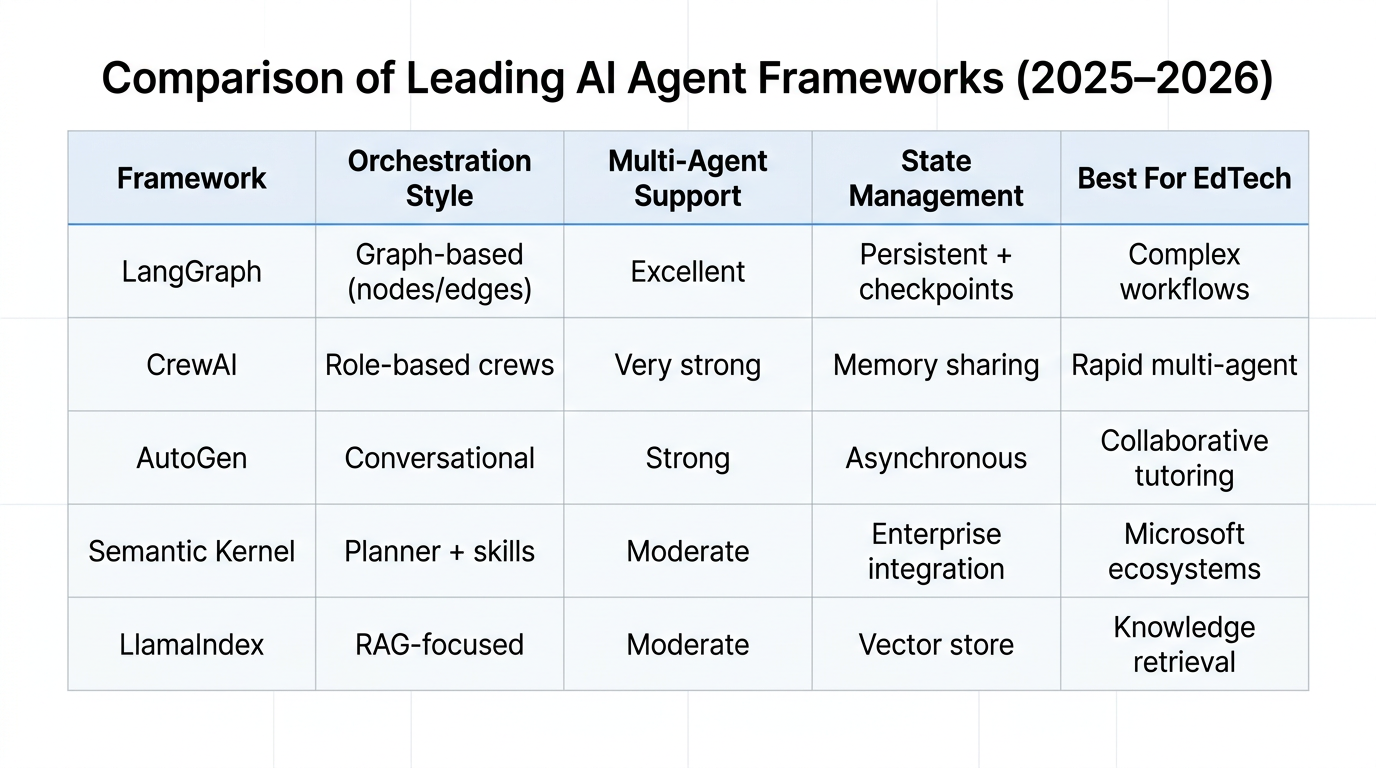
\includegraphics[width=1.0\textwidth]{generated-image.png}
  \caption{Comparaison des principaux frameworks d'agents IA (2025--2026)}
  \label{fig:frameworks-comparison}
\end{figure}

\subsection{LangGraph et environnement d'exécution basé sur des graphes}

\begin{figure}[H]
  \centering
  
\includegraphics[width=0.32\textwidth]{logo-langraph.png}
  \caption{Logo officiel de LangGraph.}
  \label{fig:langgraph-logo}
\end{figure}

LangGraph (au sein de l'écosystème LangChain) illustre l'orchestration moderne. Il
représente les workflows sous forme de graphes orientés où les nœuds sont des agents
ou des outils et les arêtes définissent le routage conditionnel. Un état persistant et
des points de contrôle avec intervention humaine garantissent la fiabilité, un aspect
critique lors de l'intégration de données étudiantes sensibles~\cite{langgraphdocs}.
Dans notre couche SprintUp, nous tirerons parti du schéma de superviseur de LangGraph
combiné à l'exposition d'outils via MCP.

Trois principaux schémas d'orchestration dominent la pratique actuelle et sont bien
pris en charge par des cadres comme LangGraph. La figure~\ref{fig:sequential} présente
le premier schéma.

%% ── Schéma 1 : Séquentiel ───────────────────────────────────
\begin{figure}[H]
\centering
\begin{tikzpicture}[
    node/.style={rectangle, rounded corners=6pt, draw, thick,
      minimum width=2.7cm, minimum height=0.8cm, align=center},
    arrow/.style={->, thick, -{Stealth[length=3mm]}}
]
\node[node, fill=gray!10, font=\bfseries] (title) {Sequential};
\node[node, below=0.8cm of title]  (q)  {User Query};
\node[node, below=0.65cm of q]     (s1) {Step 1};
\node[node, below=0.65cm of s1]    (s2) {Step 2};
\node[node, below=0.65cm of s2]    (s3) {Step 3};
\node[node, below=0.65cm of s3]    (f)  {Final Answer};
\draw[arrow] (q) -- (s1);
\draw[arrow] (s1) -- (s2);
\draw[arrow] (s2) -- (s3);
\draw[arrow] (s3) -- (f);
\end{tikzpicture}
\caption{Schéma séquentiel d'orchestration}
\label{fig:sequential}
\end{figure}

Sequential orchestration organise les tâches dans une chaîne linéaire. Chaque étape
attend la fin de la précédente avant de transmettre sa sortie. Ce schéma convient bien
à des flux de travail clairement définis, comme \og{}récupérer l'emploi du temps du
cours $\rightarrow$ extraire les notes du chapitre concerné $\rightarrow$ générer des
exercices supplémentaires\fg{}. Sa simplicité facilite le débogage, mais il peut
devenir un goulot d'étranglement lorsque des sous-tâches pourraient s'exécuter
indépendamment.

%% ── Schéma 2 : Parallèle ────────────────────────────────────
La figure~\ref{fig:parallel} présente le deuxième schéma.

\begin{figure}[H]
\centering
\begin{tikzpicture}[
    node/.style={rectangle, rounded corners=6pt, draw, thick,
      minimum width=2.7cm, minimum height=0.8cm, align=center},
    arrow/.style={->, thick, -{Stealth[length=3mm]}}
]
\node[node, fill=gray!10, font=\bfseries]     (title) {Parallel};
\node[node, below=0.55cm of title]            (q)   {User Query};
\node[node, below=0.55cm of q]                (s)   {Splitter};
\node[node, below left=0.7cm and 0.3cm of s]  (a)   {Agent 1};
\node[node, below right=0.7cm and 0.3cm of s] (b)   {Agent 2};
\node[node, below=2.9cm of s]                 (m)   {Merge};
\node[node, below=0.55cm of m]                (f)   {Final Answer};
\draw[arrow] (q) -- (s);
\draw[arrow] (s) -- (a);
\draw[arrow] (s) -- (b);
\draw[arrow] (a) -- (m);
\draw[arrow] (b) -- (m);
\draw[arrow] (m) -- (f);
\end{tikzpicture}
\caption{Schéma parallèle d'orchestration}
\label{fig:parallel}
\end{figure}

Parallel (ou simultaneous) orchestration permet à plusieurs agents ou outils de
s'exécuter en même temps. Une requête peut lancer séparément la récupération de
l'emploi du temps du jour, la recherche de ressources multimédias et la rédaction
d'un résumé ; les résultats sont ensuite fusionnés par une étape de combinaison.
Cette approche améliore la rapidité et convient particulièrement aux contextes
éducatifs où les enseignants ont besoin d'un support rapide et multiple. La difficulté
principale réside dans la résolution des conflits et la synchronisation de l'état.

%% ── Schéma 3 : Supervisé ────────────────────────────────────
La figure~\ref{fig:supervised} présente le troisième schéma.

\begin{figure}[H]
\centering
\begin{tikzpicture}[
    node/.style={rectangle, rounded corners=6pt, draw, thick,
      minimum width=2.7cm, minimum height=0.8cm, align=center},
    arrow/.style={->, thick, -{Stealth[length=3mm]}}
]
\node[node, fill=gray!10, font=\bfseries] (title) {Supervised};
\node[node, below=0.8cm of title]                (q)   {User Query};
\node[node, below=0.9cm of q]                    (sup) {Supervisor};
\node[node, below left=1.05cm and -1.0cm of sup] (sp1) {Specialist 1};
\node[node, below right=1.05cm and -1.0cm of sup](sp2) {Specialist 2};
\node[node, below=2.2cm of sup]                  (f)   {Final Answer};
\draw[arrow] (q)   -- (sup);
\draw[arrow] (sup) -- (sp1);
\draw[arrow] (sup) -- (sp2);
\draw[arrow] (sp1) -- (sup);
\draw[arrow] (sp2) -- (sup);
\draw[arrow] (sup) -- (f);
\end{tikzpicture}
\caption{Schéma supervisé (hiérarchique) d'orchestration}
\label{fig:supervised}
\end{figure}

Supervised (ou hierarchical/orchestrator-worker) orchestration introduit un agent
superviseur central qui agit comme routeur et contrôleur de qualité. Le superviseur
analyse la requête utilisateur, décide quels agents spécialisés appeler, surveille
l'avancement, puis synthétise la réponse finale. Ce schéma, bien implémenté dans les
graphes superviseur de LangGraph, reflète la gestion d'une équipe humaine et offre
de bons mécanismes de gestion d'erreur et de repli. C'est le schéma que nous
privilégierons dans notre couche SprintUp, car il équilibre flexibilité et contrôle,
ce qui est essentiel pour une intégration avec des services backend en production.

LangGraph montre comment ces schémas peuvent coexister dans un même runtime basé sur
des graphes. Les nœuds représentent des agents ou des outils, les arêtes définissent
le flux de données et le routage conditionnel, et l'état persistant avec points de
contrôle humains assure la fiabilité. Ces cadres ont fait évoluer le développement
d'agents, passant de chaînes de prompts fragiles à des workflows testables et de
niveau production.

\subsection{Approfondissement du schéma de superviseur LangGraph}

Les environnements d'exécution basés sur des graphes comme LangGraph fournissent non
seulement des schémas abstraits, mais aussi des mécanismes concrets pour construire
des systèmes multi-agents robustes. Dans une configuration typique de superviseur, un
nœud contrôleur de haut niveau reçoit la requête utilisateur, inspecte l'état courant
et décide quels agents spécialistes ou outils invoquer
ensuite~\cite{langgraphsupervisor,langgraphdocs}. Ces spécialistes peuvent inclure par
exemple un agent \og{}cours\fg{}, un agent \og{}notes\fg{} ou un générateur
d'exercices, chacun responsable d'une capacité restreinte alignée sur un service backend
spécifique.

Le modèle de graphe d'état de LangGraph permet au superviseur de maintenir une mémoire
structurée des résultats intermédiaires, des sorties d'outils et des signaux d'erreur,
ce qui facilite la replanification lorsqu'un outil échoue ou que des informations
supplémentaires sont nécessaires~\cite{ibmlanggraph}. Les mécanismes de checkpointing et
les contrôles avec humain dans la boucle, désormais standards dans les versions modernes
de LangGraph, jouent un rôle clé dans les scénarios éducatifs où des interventions
d'enseignants ou d'administrateurs peuvent être requises avant l'exécution d'actions
sensibles sur les données étudiantes~\cite{anthropicagents}. Cette combinaison de
routage supervisé, d'état persistant et de points de contrôle explicites constituera
l'ossature de la couche d'orchestration SprintUp.

%% ────────────────────────────────────────────────────────────
\section{Le Model Context Protocol (MCP) : définition, origines et justification}

Tandis que l'orchestration gouverne le flux de haut niveau, le Model Context Protocol
traite la question plus bas niveau de la communication des agents avec les systèmes
externes. Annoncé par Anthropic en novembre 2024 puis étendu via des mises à jour de
spécification ouvertes, MCP est un protocole ouvert et standardisé qui fonctionne
comme un \og{}port USB-C de l'IA\fg{}~\cite{anthropic2024,anthropicmcpdocs}.

Il définit une architecture client--serveur cohérente. Côté client,
un composant MCP intégré dans l'environnement d'exécution de l'agent
charge les descriptions d'outils et leurs capacités dans la fenêtre
de contexte du modèle. Le modèle décide alors quels outils appeler
et émet des requêtes structurées. Côté serveur, des serveurs MCP
exposent les services backend (bases de données, API, systèmes de
fichiers, fonctions métier) de façon uniforme via JSON-RPC sur des
canaux sécurisés. La spécification 2025 définit deux transports
principaux : \texttt{stdio} pour les intégrations locales et
\textbf{Streamable HTTP} (successeur du transport SSE initial) pour
les déploiements réseau ; ce dernier permet des requêtes HTTP POST
stateless avec réponses JSON directes, facilitant le passage à
l'échelle derrière un load balancer. Les résultats transitent par
le même protocole, ce qui autorise des interactions multi-tours
fluides.

À la différence des mécanismes traditionnels d'appel de fonctions
(\emph{function calling}) qui exigent du code de liaison spécifique pour
chaque nouveau service, MCP découple l'agent des
détails d'implémentation. Les développeurs implémentent le serveur MCP une seule fois
pour leur backend (dans notre cas, les endpoints de services étudiants pour les cours,
notes, génération de contenu, etc.), et tout agent conforme peut ensuite découvrir et
utiliser immédiatement ces outils. MCP a précisément été conçu pour résoudre la
fragmentation qui pénalisait les premiers développements d'agents : avant 2024, chaque
entreprise devait écrire des intégrations sur mesure pour chaque base de données, API
ou outil, un cauchemar de maintenance qui passait mal à l'échelle et introduisait des
incohérences de sécurité~\cite{anthropic2024,mcpspec}. D'un point de vue
cybersécurité, au cœur de ce programme, les hooks d'authentification intégrés au
protocole, les périmètres d'autorisation et le format de messages propice à l'audit
représentent une avancée majeure par rapport aux solutions \emph{ad hoc}
d'appel de fonctions~\cite{mcpsecurity}.

MCP ne remplace pas la récupération d'information ; il la complète. La recherche
agentique sur sources externes excelle dans la collecte de connaissances
actualisées pour ancrer le contenu généré dans des sources fiables. MCP permet à
l'agent d'agir sur ces connaissances en appelant des services applicatifs en temps réel.
Dans le contexte SprintUp, la rédaction d'une activité déclenche d'abord la
collecte du contexte pédagogique pertinent par recherche externe, puis les
outils \gls{mcp} de création et de mise à jour pour persister le contenu dans
la base de connaissances.

\subsection{Architecture détaillée et flux protocolaire}

MCP définit une architecture client--serveur basée sur JSON-RPC via des événements
envoyés par le serveur. Le client MCP (intégré dans l'exécution de l'agent) charge les
descriptions d'outils dans la fenêtre de contexte du modèle et les expose sous forme
de définitions structurées que le modèle peut appeler~\cite{anthropicmcpdocs,mcpspec}.
Quand le modèle décide d'invoquer un outil, il émet une requête JSON-RPC :

\begin{tcolorbox}[colback=gray!5, colframe=gray!50, arc=3pt,
    title={\small Exemple de requ\^{e}te JSON-RPC MCP}]
\small\ttfamily
\{``jsonrpc'': ``2.0'', ``method'': ``tools/call'',\\
\ ``params'': \{``name'': ``create\_activity'',\\
\quad``arguments'': \{``unit\_id'': ``u-01'',\\
\qquad``title'': ``Les bases de données relationnelles''\}\}\}
\end{tcolorbox}

Le serveur MCP reçoit la requête, exécute la logique backend correspondante
et renvoie une réponse structurée :

\begin{tcolorbox}[colback=gray!5, colframe=gray!50, arc=3pt,
    title={\small Exemple de r\'{e}ponse JSON-RPC MCP}]
\small\ttfamily
\{``jsonrpc'': ``2.0'', ``id'': 1,\\
\ ``result'': \{``id'': ``a-42'',\\
\quad``title'': ``Les bases de données relationnelles'',\\
\quad``position'': 0, ``status'': ``created''\}\}
\end{tcolorbox}

Le transport \textbf{\emph{Streamable HTTP}} se prête naturellement à un mode
sans état dans lequel chaque appel \gls{rpc} est auto-contenu et n'oblige pas
le serveur à mémoriser une session de
client~\cite{anthropicmcpdocs}. La figure~\ref{fig:mcp-architecture} illustre
cette architecture de haut niveau.

\begin{figure}[H]
\centering
\begin{tikzpicture}[
    node/.style={rectangle, rounded corners=6pt, draw, thick,
      minimum width=3.5cm, minimum height=1cm, align=center},
    arrow/.style={->, thick, -{Stealth[length=3mm]}}
]
\node[node] (model)  {Agent LLM};
\node[node, below=1.5cm of model]  (client) {Client MCP};
\node[node, below=1.5cm of client] (server) {Serveur MCP (Backend)};
\draw[arrow] (model)  -- node[midway,right] {Appel d'outil} (client);
\draw[arrow] (client) -- node[midway,right] {JSON-RPC}      (server);
\draw[arrow] (server) -- node[midway,left]  {Réponse}       (client);
\draw[arrow] (client) -- node[midway,left]  {Résultat}      (model);
\end{tikzpicture}
\caption{Architecture client--serveur MCP (spécification 2025)}
\label{fig:mcp-architecture}
\end{figure}

Du point de vue de l'implémentation, la spécification MCP et les implémentations de
référence dans des langages courants (Python, TypeScript) fournissent une cartographie
claire entre les capacités côté serveur et les schémas d'outils visibles dans le
contexte du modèle~\cite{anthropicmcpdocs}. Cela réduit la complexité accidentelle et
facilite la compréhension des opérations qu'un agent est autorisé à effectuer dans un
déploiement éducatif donné.

\subsection{Fonctionnalités de sécurité et risques}

Sur le plan de la cybersécurité, MCP présente plusieurs avantages par rapport aux
schémas informels d'appel de fonctions. Tout d'abord, il encourage une définition
explicite des outils disponibles et de leurs paramètres, ce qui s'aligne sur le
principe du moindre privilège : un agent interagissant avec SprintUp peut n'avoir
accès qu'à des méthodes de consultation de cours en lecture seule pour les profils
étudiants, tandis que les agents enseignants bénéficient de capacités d'écriture plus
larges~\cite{mcpsecurity}. Ensuite, les messages JSON-RPC structurés constituent une
piste d'audit naturelle pouvant être journalisée et surveillée pour détecter des
comportements suspects.

Des risques subsistent néanmoins. Des attaquants pourraient tenter d'enregistrer des
serveurs MCP malveillants exposant des outils conçus pour exfiltrer des données ou
injecter du contenu adversarial dans le contexte de l'agent. Des attaques par injection
de prompt ou empoisonnement de données peuvent également survenir via les réponses
d'outils si celles-ci ne sont pas correctement filtrées~\cite{mcpsecurity}.
Plusieurs mesures de mitigation sont recommandées. La première
consiste à exiger une authentification et une autorisation strictes
des serveurs MCP avant leur mise à disposition de l'agent. La
deuxième repose sur des périmètres fins et un contrôle d'accès basé
sur les rôles (\acrshort{rbac}) définissant les outils qu'un profil
d'utilisateur peut invoquer. La troisième impose la validation des
entrées et des sorties de tous les appels d'outils, avec filtrage
du contenu non fiable avant qu'il n'atteigne le modèle. La
quatrième, enfin, repose sur une journalisation exhaustive et une
détection d'anomalies sur le trafic MCP, en particulier pour les
opérations impliquant des données personnelles d'étudiants.

Dans l'implémentation SprintUp, ces mesures seront intégrées aux contrôles de sécurité
existants et aux politiques de protection des données.

%% ────────────────────────────────────────────────────────────
\section{État de l'art : applications en éducation}

La combinaison de l'orchestration, de la Retrieval-Augmented Generation (RAG) et
d'intégrations de type MCP a déjà donné lieu à des résultats convaincants dans des
environnements éducatifs à travers le monde. L'Arizona State University (ASU), par
exemple, a lancé en 2024 un important \og{}AI Innovation Challenge\fg{} ayant attiré
plus de 175 propositions et financé plus de 200 projets couvrant la majorité de ses
unités académiques~\cite{asu2024}. Ces initiatives incluent des agents de tutorat
personnalisé et des outils de simulation combinant RAG pour la récupération de
connaissances et des mécanismes d'orchestration pour fournir des expériences
d'apprentissage adaptatives.

De la même façon, des prototypes basés sur RAG ont montré de bonnes performances dans
les environnements universitaires. Une revue systématique récente sur RAG pour les
applications éducatives met en évidence la façon dont les modèles augmentés par la
récupération peuvent alimenter des systèmes d'apprentissage interactifs, la génération
de contenu et l'évaluation automatisée, tout en réduisant les hallucinations par rapport
aux modèles purement génératifs~\cite{rageducation,lirageducation}.

Un exemple particulièrement pertinent pour ce projet est l'expérience d'Intellect
Academy en Tunisie, qui opère via la plateforme SprintUp sur plusieurs campus et
filières de formation~\cite{intellect2025}. En intégrant l'IA pour le développement de
curricula, les parcours d'apprentissage adaptatifs et le pilotage unifié de la
performance, l'académie a accéléré la création de contenu tout en préservant une forte
maîtrise pédagogique.

L'Université Northeastern a, elle, noué un partenariat avec Anthropic pour déployer des
agents basés sur Claude sur ses campus pour le tutorat personnalisé et le support
administratif~\cite{northeastern2025,duke2025}. Ces initiatives illustrent une tendance
plus large en 2025--2026 : l'émergence d'universités \og{}IA natives\fg{} où des
systèmes agentiques soutiennent le conseil, le tutorat et les workflows d'alerte
précoce à grande échelle~\cite{agenticragsurvey,agenticrag2025}.

\subsection{RAG agentique pour l'apprentissage personnalisé}

Les pipelines classiques de Retrieval-Augmented Generation (RAG) récupèrent un ensemble
statique de documents à partir de la requête utilisateur, puis génèrent une réponse en
un seul passage. Si cela améliore l'ancrage factuel, ces workflows peuvent rencontrer
des difficultés pour le raisonnement multi-étapes, les questions ambiguës ou les tâches
nécessitant une exploration adaptative de la base de
connaissances~\cite{lewis2020,rageducation}. Le RAG agentique étend ce paradigme en
intégrant des agents autonomes dans la chaîne RAG. Ces agents s'appuient sur des
schémas de conception tels que la planification, la réflexion, l'utilisation d'outils
et la collaboration multi-agents pour piloter dynamiquement les stratégies de
récupération, affiner itérativement le contexte et adapter les
workflows~\cite{agenticragsurvey}.

Dans des scénarios d'apprentissage personnalisé, un système de RAG
agentique peut ainsi planifier une séquence de récupérations à
partir de notes de cours, de chapitres de manuels et d'anciens
sujets d'examen, puis réfléchir à la suffisance du contexte
récupéré et émettre des requêtes complémentaires en cas de lacunes.
Il peut également utiliser des outils pour parcourir des graphes
de connaissances ou interroger un modèle de l'étudiant afin
d'adapter les explications à son niveau actuel.

La revue consacrée à RAG pour les applications éducatives met spécifiquement en avant
quatre grands schémas d'application : systèmes de questions--réponses éducatifs,
chatbots pédagogiques, systèmes de tutorat pilotés par IA et parcours d'apprentissage
adaptatifs~\cite{rageducation,lirageducation}. Chacun de ces schémas s'aligne
étroitement avec les services backend existants de SprintUp.

%% ────────────────────────────────────────────────────────────
\section{Conclusion du chapitre}

Ce chapitre a posé les bases conceptuelles : l'orchestration fournit l'intelligence de
coordination des tâches complexes, tandis que MCP apporte la plomberie standardisée et
sécurisée qui connecte les agents aux systèmes backend réels. Combinées à RAG (détaillé
dans les chapitres suivants), ces technologies constituent la pile complète nécessaire
pour concrétiser notre vision pour SprintUp. Les schémas et les protocoles présentés ici
ne sont pas théoriques ; ils adressent directement le déficit d'intégration mis en
évidence en introduction et orienteront chacune des décisions de conception à venir.

\subsection{Synthèse et lien avec SprintUp}

Le schéma d'orchestration supervisée, combiné à l'exposition d'outils via MCP et à
l'ancrage par RAG, s'ajuste naturellement aux services backend de SprintUp. L'analyse de
la sécurité de MCP et de l'orchestration d'agents présentée dans ce chapitre fournit un
socle pour concevoir une couche d'agents conformes et auditables, respectant la vie
privée des étudiants et les contraintes institutionnelles. Forts de ces fondations, nous
pouvons désormais passer à l'implémentation concrète de la récupération d'information,
de l'exposition des outils via MCP et de la logique d'orchestration dans les chapitres
de mise en \oe{}uvre qui suivent.
\newpage


%% Chapitre 2 — Conception de la couche d'agents
%% ============================================================
%%  CHAPITRE 2 — Conception de la couche d'agents
%% ============================================================
\chapter{Conception de la couche d'agents}
\label{chap:conception}

%% Listes d'outils \mcptool{...} très denses : ouvrir les marges
%% intérieures pour autoriser les coupures à _ , ( etc.
\sloppy

L'introduction a posé le problème (redondance, absence d'ancrage factuel,
absence de séparation des privilèges) et le chapitre~1 a établi les fondations
théoriques : orchestration d'agents, Model Context Protocol et \gls{rag}
agentique. Le présent chapitre traduit ces fondations en une conception logique
complète, puis relit les implémentations livrées comme un \emph{catalogue
comparé de formes d'agents}. Il prépare ainsi la stratégie d'orchestration qui
fera l'objet du chapitre~3.

La première partie traite de l'indexation des activités, pierre angulaire sans
laquelle la non-redondance ne serait qu'un v{\oe}u. La deuxième présente le
protocole \gls{mcp} tel qu'il s'applique au système, avec le catalogue d'outils
qu'il expose et le principe du moindre privilège qui gouverne leur
distribution. La troisième détaille le catalogue des agents retenus, en
réservant une matrice à quatre variantes pour l'agent de création de syllabus.
La quatrième propose une lecture comparative des implémentations : non un test
de conformité, mais un examen architectural de ce que chaque variante
privilégie et de ce qu'elle paie en contrepartie. La conclusion enchaîne sur le
chapitre~3, en montrant que ces différences de conception appellent une
stratégie d'orchestration de niveau supérieur.

%% ────────────────────────────────────────────────────────────
\section{Indexation des activités pédagogiques}
\label{sec:indexation}

\subsection{Le problème de la redondance}

L'approche mono-modèle décrite en introduction souffre d'un défaut structurel :
chaque appel au \gls{llm} produit du contenu nouveau sans mémoire de ce qui a
déjà été produit. Sur un parcours pédagogique enrichi au fil de plusieurs
sessions, plusieurs activités finissent par traiter le même concept sous des
angles à peine différents.

Cette redondance n'est pas qu'un problème esthétique. Elle dilue l'ancrage des
objectifs d'apprentissage, alourdit la charge cognitive de l'apprenant et
complique le travail de l'enseignant qui doit trier manuellement les doublons.
Pour qu'un agent génère du contenu utile, il doit d'abord savoir ce qui existe.

La solution retenue est un mécanisme d'indexation qui transforme chaque
activité existante en une représentation numérique comparable, et qui expose
une opération de recherche par similarité aux agents générateurs.
L'indexation constitue la pierre angulaire du système : sans elle, les parties
suivantes (\gls{mcp}, agents) perdraient leur raison d'être.

\subsection{Représentation vectorielle des activités}

Le principe est le suivant. Chaque activité pédagogique (cours, question,
exercice ou quiz) est décrite par un texte : son titre concaténé avec son
contenu. Ce texte est transformé en un vecteur numérique de dimension fixe
par un modèle de plongement (\emph{embedding model}). La dimension du vecteur
est déterminée par le modèle retenu ; elle est sans incidence sur la logique
de l'agent, qui ne manipule jamais les composantes individuelles. Deux textes
sémantiquement proches, par exemple deux exercices portant sur la résolution
d'équations du second degré, produisent des vecteurs proches dans cet espace,
même si leur formulation diffère.

\begin{figure}[H]
\centering
\begin{tikzpicture}[
    node/.style={rectangle, rounded corners=6pt, draw, thick,
      minimum width=3.0cm, minimum height=1.0cm, align=center},
    arrow/.style={->, thick, -{Stealth[length=3mm]}}
]
\node[node, fill=myblue!8] (txt) {Titre + contenu\\de l'activité};
\node[node, right=1.5cm of txt, fill=myblue!8] (emb) {Modèle de\\plongement};
\node[right=1.6cm of emb] (vec) {$\vec{v}\in\mathbb{R}^{d}$};
\draw[arrow] (txt) -- (emb);
\draw[arrow] (emb) -- (vec);
\end{tikzpicture}
\caption{Transformation d'une activité en vecteur numérique.}
\label{fig:embedding}
\end{figure}

À partir de cette représentation, le système définit une \textbf{mesure de
similarité} entre deux activités. Soit $\vec{u}$ le vecteur d'une activité
existante et $\vec{v}$ celui d'un brouillon à créer ; la similarité
$s(\vec{u}, \vec{v})$ est une fonction qui croît lorsque les deux vecteurs
pointent dans la même direction de l'espace de plongement, et qui décroît
lorsqu'ils en divergent. Le choix précis de cette mesure (cosinus, distance
euclidienne ou autre) relève de la configuration du moteur d'indexation et
non de la conception de l'agent.

Une calibration de cette similarité — un point au-delà duquel deux activités
sont considérées comme un quasi-doublon — peut être fixée côté serveur de
manière empirique. Cette calibration reste un paramètre d'implémentation~:
elle n'appartient pas au contrat de l'agent, qui consomme la primitive de
recherche sans en connaître les constantes. Le chapitre ne fait donc pas
reposer son argumentaire sur une valeur numérique particulière~; ce sont les
\emph{propriétés} de la recherche par similarité (ordonnancement par
proximité, signal complémentaire de la lecture directe) qui structurent la
conception.

\subsection{Pipeline d'indexation}
\label{sec:pipeline-index}

Le pipeline d'indexation comporte deux flux complémentaires : la
\textbf{création} d'un index à partir des activités existantes, et la
\textbf{recherche} par similarité avant chaque nouvelle écriture.

\begin{figure}[H]
\centering
\begin{tikzpicture}[
    node/.style={rectangle, rounded corners=5pt, draw, thick,
      minimum width=3.0cm, minimum height=0.8cm, align=center,
      font=\small},
    db/.style={cylinder, draw, thick, shape border rotate=90,
      aspect=0.3, minimum height=1.2cm, minimum width=1.8cm,
      align=center, font=\small, fill=myblue!8},
    arrow/.style={->, thick, -{Stealth[length=3mm]}}
]
%% Flux gauche : création de l'index
\node[node, fill=myblue!8] (act) {Activité\\(titre + contenu)};
\node[node, below=0.7cm of act, fill=myblue!8] (mod1) {Modèle de\\plongement};
\node[db, below=0.7cm of mod1] (db1) {Index\\vectoriel};
\draw[arrow] (act) -- (mod1);
\draw[arrow] (mod1) -- (db1);
\node[above=0.15cm of act, font=\bfseries\small] {Création};

%% Flux droite : recherche
\node[node, right=3.0cm of act, fill=myblue!8] (q) {Requête\\(sujet)};
\node[node, below=0.7cm of q, fill=myblue!8] (mod2) {Modèle de\\plongement};
\node[node, below=0.7cm of mod2, fill=myblue!8] (sim)
  {Recherche par\\similarité ($k$-NN)};
\node[node, below=0.7cm of sim, fill=myblue!8] (res)
  {Top-$k$ activités\\les plus proches};
\draw[arrow] (q) -- (mod2);
\draw[arrow] (mod2) -- (sim);
\draw[arrow] (sim) -- (res);
\draw[arrow] (db1) -- node[above, font=\footnotesize]{interroge} (sim);
\node[above=0.15cm of q, font=\bfseries\small] {Recherche};
\end{tikzpicture}
\caption{Pipeline d'indexation : création (gauche) et recherche (droite).}
\label{fig:pipeline}
\end{figure}

À la création, chaque nouvelle activité passe par le modèle de plongement et
le vecteur résultant est persisté dans un index vectoriel aux côtés de
l'identifiant de l'activité. À la recherche, la requête de l'agent (typiquement
le sujet d'une activité à créer) est elle-même plongée, puis comparée à toutes
les entrées de l'index ; les $k$ plus proches sont retournées avec leur score
de similarité.

\subsection{Place de l'indexation dans l'architecture}

L'indexation n'est pas un service autonome que les agents appellent
directement. Elle est encapsulée dans le serveur \gls{mcp} sous la forme
d'outils de recherche sémantique typés, accompagnés d'une mise à jour
automatique de l'index à chaque création d'activité ou d'unité. L'agent ne
voit donc l'indexation qu'à travers deux interfaces : une opération de
recherche par similarité, en lecture, et une persistance enrichie de
l'indexation, en écriture.

Deux niveaux d'usage de cette indexation se distinguent dans la conception
du système.

Le premier niveau est l'usage \textbf{intra-syllabus}. Lorsqu'un agent doit
produire une nouvelle activité dans un syllabus existant, son premier réflexe
est la \textbf{lecture directe} des unités et activités sœurs : il interroge
le serveur \gls{mcp} pour lister la structure du syllabus, puis lit le corps
des activités voisines pour comprendre ce qui a déjà été enseigné. Cette
lecture de proximité, déterministe et peu coûteuse, porte l'essentiel de la
non-redondance dans le périmètre d'une seule unité. La recherche par
similarité y joue le rôle de \textbf{signal complémentaire} : elle permet de
détecter un quasi-doublon sémantique que la simple comparaison de titres
n'aurait pas révélé, ou de signaler qu'une activité jugée nouvelle reformule
en réalité un contenu existant.

Le second niveau est l'usage \textbf{global}, où la lecture directe ne peut
plus suffire. Trois situations le réclament. D'abord, la création d'un
\textbf{nouveau syllabus} : pour éviter qu'un enseignant ne produise un
doublon d'un syllabus existant dans la base, l'agent doit pouvoir interroger
l'ensemble du catalogue par similarité, et pas seulement la liste textuelle
des titres. Ensuite, l'\textbf{agent assistant élève} : lorsqu'un apprenant
est bloqué sur un concept, l'agent doit pouvoir retrouver les activités
sémantiquement proches à recommander, indépendamment de l'unité courante.
Enfin, l'\textbf{agent tuteur} : pour proposer des variantes pédagogiques ou
du matériel d'appui, l'agent doit pouvoir retrouver dans l'ensemble du
catalogue les activités voisines d'une activité donnée.

C'est sur ces trois usages que repose la valeur structurante de l'indexation.
Elle reste accessible au niveau intra-syllabus comme garde-fou anti-doublon,
mais son rôle décisif se déploie à l'échelle globale, dès que les agents
doivent raisonner au-delà du périmètre d'un seul syllabus.

%% ────────────────────────────────────────────────────────────
\section{Le protocole MCP appliqué au système}
\label{sec:mcp-systeme}

\subsection{Rappel : qu'est-ce que le MCP}

Le Model Context Protocol (\gls{mcp}), introduit en détail au chapitre~1, est
un protocole ouvert qui standardise la façon dont un agent \gls{llm} découvre
et appelle des outils fournis par un serveur externe~\cite{anthropic2024,mcpspec}.
Son architecture client--serveur repose sur \gls{json}-\gls{rpc} : le client
(intégré dans le runtime de l'agent) charge les descriptions d'outils, le
modèle décide lesquels appeler, et le serveur exécute la logique
correspondante puis renvoie un résultat structuré.

Deux propriétés du protocole sont particulièrement pertinentes pour
le présent système. La première est la \emph{découverte automatique} :
un agent conforme peut interroger un serveur \gls{mcp} pour obtenir
la liste de ses outils, y compris leurs schémas d'entrée et leur
documentation, ce qui permet d'ajouter un nouvel outil au serveur
sans modifier le code de l'agent — un simple redémarrage de la
connexion suffit. La seconde est le \emph{découplage entre l'agent
et son backend} : l'agent ne connaît ni la base de données ni le
langage du serveur, mais seulement des noms d'outils et des schémas
\gls{json}, ce qui permet de faire évoluer le backend (changer de
\gls{bd}, ajouter un cache) sans impacter les agents qui le
consomment.

\subsection{Architecture MCP du système}
\label{sec:mcp-archi}

Le système expose trois serveurs \gls{mcp}, chacun couvrant un domaine
fonctionnel distinct (figure~\ref{fig:mcp-servers}).

\begin{figure}[H]
\centering
\begin{tikzpicture}[
    server/.style={rectangle, rounded corners=5pt, draw, thick,
      minimum width=3.0cm, minimum height=1.0cm, align=center,
      fill=myblue!10, font=\small\bfseries},
    consumer/.style={rectangle, rounded corners=5pt, draw, thick,
      minimum width=3.0cm, minimum height=0.9cm, align=center,
      fill=gray!8, font=\small},
    arrow/.style={->, thick, -{Stealth[length=3mm]}, gray!70}
]
\node[server] (s1) {Serveur MCP\\Curriculum};
\node[server, right=0.8cm of s1] (s2) {Serveur MCP\\Données étudiants};
\node[server, right=0.8cm of s2] (s3) {Serveur MCP\\Analytique};

\node[consumer, below=1.5cm of s1] (c1)
  {Agents\\générateurs};
\node[consumer, below=1.5cm of s2] (c2)
  {Tuteur /\\Assistant élève};
\node[consumer, below=1.5cm of s3] (c3)
  {Assistant\\administrateur};

\draw[arrow] (s1) -- (c1);
\draw[arrow] (s2) -- (c2);
\draw[arrow] (s3) -- (c3);
\end{tikzpicture}
\caption{Trois serveurs MCP et les agents qui les consomment.}
\label{fig:mcp-servers}
\end{figure}

Le \emph{Serveur Curriculum} expose la hiérarchie syllabus
$\rightarrow$ unité $\rightarrow$ activité ; il constitue le serveur
principal du système, en cela que tous les agents générateurs le
consomment et que l'indexation vectorielle y est directement
intégrée. Le \emph{Serveur Données étudiants} expose les
soumissions, la progression et les retours ; il est consommé par le
tuteur, en lecture comme en écriture de feedback, et par
l'assistant élève, en lecture seule. Le \emph{Serveur Analytique}
expose enfin les rapports agrégés d'inscription, de complétion et
d'empreinte de contenu ; il est consommé par l'assistant
administrateur.

Chaque serveur supporte deux modes de transport conformes à la
spécification \gls{mcp} 2025~\cite{mcpspec}. En mode \emph{stdio},
le processus \gls{api} lance le serveur \gls{mcp} comme processus
enfant : ce mode est adapté au développement local, sans aucune
configuration réseau. En mode \emph{Streamable HTTP}, le serveur
\gls{mcp} tourne comme service indépendant derrière un domaine
privé ; chaque appel \gls{json}-\gls{rpc} prend la forme d'une
requête \gls{http} POST sans état, ce qui rend possible le passage
à l'échelle derrière un répartiteur de charge.

\subsection{Catalogue d'outils MCP}
\label{sec:mcp-catalogue}

Le tableau~\ref{tab:mcp-curriculum} énumère l'ensemble des outils exposés par
le serveur Curriculum. La distinction lecture / écriture est structurante :
les outils de lecture retournent des métadonnées légères (identifiants,
titres, ordre), tandis que les outils d'écriture effectuent exactement une
mutation et retournent la ligne insérée.

\begin{table}[H]
\centering
\caption{Outils MCP du serveur Curriculum.}
\label{tab:mcp-curriculum}
\small
\begin{tabularx}{\linewidth}{@{}>{\raggedright\arraybackslash}p{4.8cm}
    >{\raggedright\arraybackslash}p{1.6cm} X@{}}
\toprule
\textbf{Outil} & \textbf{Mode} & \textbf{Description}\\
\midrule
\mcptool{list_syllabuses}            & Lecture  & Liste des syllabus (id, titre, matière).\\
\mcptool{get_syllabus}               & Lecture  & Syllabus complet avec unités et activités.\\
\mcptool{list_unities}               & Lecture  & Unités d'un syllabus (id, titre, ordre).\\
\mcptool{list_activities_for_unity}  & Lecture  & Activités d'une unité (métadonnées légères).\\
\mcptool{get_activity}               & Lecture  & Corps complet d'une activité.\\
\mcptool{find_related_unities}       & Lecture  & Recherche sémantique d'unités voisines (par plongement).\\
\mcptool{find_related_activities}    & Lecture  & Recherche sémantique d'activités voisines (par plongement).\\
\addlinespace
\mcptool{create_syllabus}        & Écriture & Crée un syllabus.\\
\mcptool{create_unity}           & Écriture & Crée une unité dans un syllabus.\\
\mcptool{create_activity}        & Écriture & Crée une activité dans une unité (avec indexation automatique).\\
\mcptool{update_unity}           & Écriture & Met à jour le titre, l'ordre ou les objectifs d'une unité.\\
\mcptool{update_activity}        & Écriture & Met à jour le corps ou les métadonnées d'une activité.\\
\addlinespace
\multicolumn{3}{@{}l@{}}{\textit{Outils ajoutés pour la Version 2 (atelier formulaire) :}}\\
\mcptool{get_unit}                       & Lecture  & Lit une unité V2 (titre, brief, syllabus parent).\\
\mcptool{list_unit_activities}           & Lecture  & Liste les activités d'une unité filtrées par statut (clé de la règle anti-redite \og référencer, ne pas redire \fg{}).\\
\mcptool{create_unit_activity}           & Écriture & Persiste une activité V2 (\mcptool{markdown} + \mcptool{activity_json}).\\
\mcptool{update_unit_activity_status}    & Écriture & Fait transiter l'activité dans la machine d'état (figure~\ref{fig:v2-status}).\\
\bottomrule
\end{tabularx}
\end{table}

Les tableaux~\ref{tab:mcp-etudiants} et~\ref{tab:mcp-analytique} listent
respectivement les outils du serveur Données étudiants et du serveur
Analytique.

\begin{table}[H]
\centering
\caption{Outils MCP du serveur Données étudiants.}
\label{tab:mcp-etudiants}
\small
\begin{tabularx}{\linewidth}{@{}>{\raggedright\arraybackslash}p{4.8cm}
    >{\raggedright\arraybackslash}p{1.6cm} X@{}}
\toprule
\textbf{Outil} & \textbf{Mode} & \textbf{Description}\\
\midrule
\mcptool{get_submissions}       & Lecture  & Soumissions d'un étudiant (filtre optionnel par activité).\\
\mcptool{get_student_progress} & Lecture  & Progression d'un étudiant dans un syllabus.\\
\mcptool{save_feedback}         & Écriture & Persiste un retour correctif sur une soumission.\\
\bottomrule
\end{tabularx}
\end{table}

\begin{table}[H]
\centering
\caption{Outils MCP du serveur Analytique.}
\label{tab:mcp-analytique}
\small
\begin{tabularx}{\linewidth}{@{}>{\raggedright\arraybackslash}p{4.8cm}
    >{\raggedright\arraybackslash}p{1.6cm} X@{}}
\toprule
\textbf{Outil} & \textbf{Mode} & \textbf{Description}\\
\midrule
\mcptool{get_enrollment_report} & Lecture & Totaux inscriptions étudiants / syllabus.\\
\mcptool{get_completion_report} & Lecture & Nombre de soumissions et score moyen.\\
\mcptool{get_content_report}    & Lecture & Empreinte de contenu (syllabus, unités, activités).\\
\mcptool{get_user_stats}        & Lecture & Répartition par rôle.\\
\mcptool{list_students}          & Lecture & Liste des étudiants.\\
\bottomrule
\end{tabularx}
\end{table}

\subsection{Principe du moindre privilège}
\label{sec:moindre-privilege}

Chaque agent ne reçoit qu'un sous-ensemble des outils \gls{mcp}, strictement
nécessaire à son rôle. Cette discipline matérialise le \textbf{principe du
moindre privilège} : un agent qui n'a pas besoin d'écrire ne dispose d'aucun
outil d'écriture, ce qui élimine par construction toute mutation
accidentelle.

Le tableau~\ref{tab:whitelist} présente la liste blanche d'outils par agent.

\begin{table}[H]
\centering
\caption{Liste blanche d'outils MCP par agent.}
\label{tab:whitelist}
\small
\begin{tabularx}{\linewidth}{@{}>{\raggedright\arraybackslash}p{4.6cm} X@{}}
\toprule
\textbf{Agent} & \textbf{Outils autorisés}\\
\midrule
Générateur d'activités\newline(sans MCP) &
  Aucun outil \gls{mcp} : génère à partir de ses connaissances uniquement.\\
\addlinespace
Générateur d'activités\newline(avec MCP) &
  \mcptool{get_syllabus},\,
  \mcptool{list_unities},\,
  \mcptool{list_activities_for_unity},\,
  \mcptool{get_activity},\,
  \mcptool{find_related_activities},\,
  \mcptool{find_related_unities},\,
  \mcptool{create_activity},\,
  \mcptool{update_activity}\\
\addlinespace
Générateur de syllabus &
  \mcptool{list_syllabuses},\,
  \mcptool{get_syllabus},\,
  \mcptool{create_syllabus},\,
  \mcptool{list_unities},\,
  \mcptool{create_unity},\,
  \mcptool{update_unity}\\
\addlinespace
Tuteur &
  \mcptool{get_activity},\,
  \mcptool{list_activities_for_unity},\,
  \mcptool{find_related_activities},\,
  \mcptool{get_student_progress},\,
  \mcptool{get_submissions},\,
  \mcptool{save_feedback}\\
\addlinespace
Assistant élève &
  \mcptool{get_syllabus},\,
  \mcptool{list_unities},\,
  \mcptool{list_activities_for_unity},\,
  \mcptool{get_activity},\,
  \mcptool{find_related_activities},\,
  \mcptool{get_student_progress}\\
\addlinespace
Assistant administrateur &
  \mcptool{get_enrollment_report},\,
  \mcptool{get_completion_report},\,
  \mcptool{get_content_report},\,
  \mcptool{get_user_stats},\,
  \mcptool{list_students},\,
  \mcptool{list_syllabuses}\\
\bottomrule
\end{tabularx}
\end{table}

Trois observations méritent d'être soulignées. L'agent~1, qui sert
de générateur d'activités sans \gls{mcp}, ne dispose d'aucun outil
exposé par le protocole : sa production, non ancrée dans le contenu
existant, constitue la ligne de base à laquelle est comparée celle
de l'agent~2 dans la lecture comparative de la
\textsection\ref{sec:comparatif}. L'assistant élève, pour sa
part, ne dispose d'aucun outil d'écriture : il peut consulter le
syllabus et la progression de l'étudiant, mais ne peut ni créer de
contenu ni modifier de données. L'assistant administrateur, enfin,
n'a accès qu'à des outils de lecture agrégée : il ne voit jamais ni
le contenu individuel des activités, ni les soumissions détaillées,
ce qui matérialise concrètement le principe du moindre privilège au
niveau de la couche d'agents.

%% ────────────────────────────────────────────────────────────
\section{Catalogue des agents}
\label{sec:catalogue-agents}

La première itération de la couche d'agents livrée à la plateforme
SprintUp comportait cinq agents coordonnés par un orchestrateur unique
et une seule interface de création de syllabus, de nature
conversationnelle. Pour valider expérimentalement le compromis
\emph{ergonomie-temps de génération-contrôlabilité} à l'échelle de
SprintUp, nous avons développé trois variantes supplémentaires du même
agent~3 (création de syllabus). Ces quatre implémentations partagent le
même contrat fonctionnel mais reposent sur deux choix d'architecture
indépendants : (i)~le \emph{mode d'interaction utilisateur} et (ii)~la
\emph{stratégie d'orchestration} interne. Cette section présente d'abord
ces deux axes (\textsection\ref{sec:axes}), puis détaille les agents
communs aux deux modes d'interaction (générateurs d'activités, tuteur,
assistant élève, assistant administrateur), et termine sur l'agent~3
décliné en quatre variantes selon les six rubriques normalisées :
identité, outils, workflow, schéma de sortie, barre de qualité et
règles.

\subsection{Cadre d'analyse : modes d'interaction et stratégies
d'orchestration}
\label{sec:axes}

Les quatre variantes de l'agent~3 proposées à l'équipe SprintUp se
lisent comme le croisement de deux axes orthogonaux. Chaque axe répond
à une question d'intégration distincte ; nous justifions chacune
brièvement avant de présenter la matrice synthétique de la
figure~\ref{fig:matrice-agents}.

\paragraph{Axe~1 — Mode d'interaction utilisateur.}
Le premier axe désigne l'interface par laquelle un enseignant de
SprintUp déclenche la création d'un syllabus. Dans la Version~1, dite
\emph{interaction conversationnelle}, l'enseignant dialogue avec
l'agent dans un fil de discussion ; un protocole de streaming typé
lui livre les artefacts (plan, unités, leçons) au fur et à mesure
de leur production, et les questions de l'agent prennent la forme
d'\emph{interruptions} structurées (formulaire d'intake, demandes
de clarification). Cette variante adopte ainsi le paradigme
\emph{Human-in-the-Loop} (\gls{hitl}), qui autorise l'enseignant à
corriger une dérive en cours de génération. La Version~2, dite
\emph{interaction par atelier formulaire}, fait au contraire reposer
le déclenchement sur un formulaire structuré (titre, description,
audience, portée horaire, intention pédagogique) : l'enseignant crée
manuellement les unités et leurs activités sous forme de
\emph{brouillons}, puis déclenche explicitement la génération. Aucun
streaming de tokens ni interruption ne se produit en cours
d'exécution ; la progression d'une activité est uniquement exposée
par une machine d'état publique (figure~\ref{fig:v2-status}), ce qui
rend la surface consommable par un client externe sans avoir à
interpréter le protocole de streaming de la Version~1.

\paragraph{Axe~2 — Stratégie d'orchestration interne.}
Le second axe décrit la manière dont la couche d'agents organise,
en interne, les quatre phases canoniques d'un travail de
curation pédagogique — rechercher, planifier, rédiger et critiquer.
Dans l'\emph{orchestration monolithique} (Option~1), un graphe d'état
figé enchaîne ces phases dans un ordre prédéfini et un unique
superviseur prend toutes les décisions de routage : le flot y gagne
en lisibilité et en reproductibilité, au prix d'une moindre
spécialisation par phase. Dans l'\emph{orchestration par sous-agents
spécialistes} (Option~2), un superviseur délègue au contraire chaque
phase à un sous-agent porteur d'une instruction système dédiée
(planner, writer, activity-maker, critic) ; la communication entre
sous-agents passe alors soit par un \gls{vfs} partagé (canal
documentaire), soit par un ordonnanceur \textsc{TypeScript} pur
(canal d'invocation). Le flot gagne en spécialisation par rôle, mais
au prix d'une coordination plus riche à mettre en place et à
maintenir.

\paragraph{Synthèse : matrice des quatre variantes.}
La figure~\ref{fig:matrice-agents} présente le croisement des deux
axes ; les quatre variantes apparaissent comme les cellules du
tableau, identifiées par le nom de code de leur composant principal
dans le dépôt : \mcptool{syllabus-generator} (V1/Op1),
\mcptool{deepagent} (V1/Op2), \mcptool{unit-bulk-supervisor} associé à
\mcptool{unit-activity-generator} (V2/Op1) et
\mcptool{sdk-orchestrator} (V2/Op2). Les quatre sous-sections de
l'agent~3 (\textsection\ref{sec:agent3}) détaillent ensuite chacune
de ces variantes selon les six rubriques normalisées.

\begin{figure}[H]
\centering
\begin{tikzpicture}[
  font=\small,
  colhead/.style={font=\small\bfseries, align=center,
                  text width=5.4cm},
  rowhead/.style={font=\small\bfseries, align=center,
                  text width=2.8cm, rotate=90},
  cell/.style ={rectangle, rounded corners=4pt, draw=myblue!60,
                line width=0.6pt, fill=myblue!5,
                minimum width=5.6cm, minimum height=2.9cm,
                text width=5.2cm, inner sep=4pt,
                align=center, font=\footnotesize},
]

%% --- axe horizontal (modes d'interaction) ---
\node[colhead] (h1) at (0, 3.25) {V1 — Interaction\\conversationnelle};
\node[colhead] (h2) at (6.4, 3.25) {V2 — Interaction par\\atelier formulaire};

%% --- axe vertical (stratégie d'orchestration) ---
\node[rowhead] (r1) at (-4.6, 0.6)  {Op.~1\\Orchestration\\monolithique};
\node[rowhead] (r2) at (-4.6, -2.7) {Op.~2\\Sous-agents\\spécialistes};

%% --- cellules ---
\node[cell] (c11) at (0, 0.6)
  {{\bfseries\color{myblue!80!black}\texttt{syllabus-generator}}\\[2pt]
   superviseur à cinq actions\\
   (intake, search, ask, write, reply)\\[2pt]
   sous-graphe \emph{search} parallèle\\
   + portail critique sévérité-sensible};

\node[cell] (c12) at (6.4, 0.6)
  {{\bfseries\color{myblue!80!black}\texttt{sdk-orchestrator}}\\[2pt]
   planificateur \textsc{LLM}\\
   $\rightarrow$ fan-out \texttt{Send}\\
   $\rightarrow$ rédacteur par unité\\[2pt]
   unités en parallèle,\\
   activités en séquence};

\node[cell] (c21) at (0, -2.7)
  {{\bfseries\color{myblue!80!black}\texttt{deepagent}}\\[2pt]
   superviseur \emph{deepagents}\\
   + 4 sous-agents : planner /\\
   writer / activity-maker / critic\\[2pt]
   communication par\\
   \textsc{VFS} partagé};

\node[cell] (c22) at (6.4, -2.7)
  {{\bfseries\color{myblue!80!black}\texttt{unit-bulk-supervisor}}\\[2pt]
   + \texttt{unit-activity-generator}\\
   + \texttt{unit-suggestion},\\
   \texttt{activity-suggestion}\\[2pt]
   brouillons +\\
   vagues de dépendances};
\end{tikzpicture}
\caption{Quatre variantes de l'agent~3 proposées pour SprintUp,
  positionnées au croisement du mode d'interaction utilisateur
  (Version~1 vs.\ Version~2) et de la stratégie d'orchestration
  (monolithique vs.\ sous-agents spécialistes). Chaque cellule porte
  le nom de code de la variante dans le dépôt et résume son schéma
  d'orchestration.}
\label{fig:matrice-agents}
\end{figure}

\paragraph{Canaux d'inter-communication.}
Les trois schémas d'orchestration distincts font apparaître trois
canaux d'inter-communication entre composants, dont la nature
conditionne directement le coût d'intégration dans SprintUp.
En V1/Op.~1 (\mcptool{syllabus-generator}), les agents ne
communiquent pas directement entre eux : toute coordination passe
par l'orchestrateur \textsc{LLM} unique, qui décide à chaque tour
quelle action exécuter et porte donc, à lui seul, l'intégralité de
la logique de routage. En V1/Op.~2 (\mcptool{deepagent}), c'est un
\gls{vfs} partagé qui sert de canal documentaire entre sous-agents
(\mcptool{/pedagogy\_plan.md}, \mcptool{/lessons/<id>.md},
\mcptool{/activities/<id>.json}, \mcptool{/critiques/<target>.md})~:
chaque sous-agent lit le travail des précédents et y ajoute le sien,
ce qui rend les artefacts inspectables a posteriori. En Version~2
enfin, il n'existe plus d'orchestrateur \textsc{LLM} de niveau
\emph{supervisor} : l'ordonnancement est intégralement délégué à du
code \textsc{TypeScript} — soit le \mcptool{unit-bulk-supervisor}
de la V2/Op.~1, qui exécute les activités par vagues de dépendances,
soit l'orchestrateur \gls{sdk} de la V2/Op.~2, qui exécute les
unités en parallèle au moyen de la primitive \mcptool{Send} de
LangGraph. Cette distinction n'est pas qu'esthétique : elle dicte si
SprintUp peut auditer l'orchestration via du code (Version~2) ou
seulement via des traces \textsc{LLM} (Version~1).

\subsection{Agent 1 : Générateur d'activités sans MCP}
\label{sec:agent1}

\paragraph{Identité.} Agent de génération d'activités pédagogiques pour la
plateforme SprintUp. Produit une ou plusieurs activités (cours, question,
exercice ou quiz) pour un sujet et une audience donnés, \emph{sans consulter
le contenu existant}. Cet agent constitue la ligne de base du système : son
fonctionnement repose entièrement sur les connaissances du modèle de langue
sous-jacent et sur les paramètres fournis dans la requête.

\paragraph{Outils.} Aucun outil \gls{mcp}, aucune recherche documentaire
externe, aucune lecture de la base de données de la plateforme. L'agent
répond à partir du seul prompt utilisateur. Cette absence délibérée en fait
le référent de comparaison pour apprécier la valeur ajoutée du \gls{mcp} et
de l'indexation au niveau de l'agent~2.

\paragraph{Workflow.}
Le déroulé est simple en quatre temps. L'agent commence par
identifier dans la requête l'ensemble des paramètres utiles — sujet,
niveau d'audience, type d'activité souhaité, nombre d'éléments,
difficulté cible et langue. Il planifie ensuite mentalement la
courbe de difficulté sur l'ensemble des activités demandées, de
manière à éviter une croissance monotone ou un palier inutile.
Vient alors la rédaction proprement dite : chaque activité est
rédigée en variant délibérément sa formulation et son niveau de
Bloom par rapport à la précédente, afin d'éviter la répétition.
L'agent termine en retournant un tableau \gls{json} dont chaque
objet décrit une activité complète.

\paragraph{Schéma de sortie.} Tableau \gls{json} d'objets \texttt{Activity} :
\mcptool{title}, \mcptool{activity_type} (\texttt{course}, \texttt{question},
\texttt{exercise}, \texttt{quiz}), \mcptool{content}, \mcptool{description},
\mcptool{difficulty} (1--5), \mcptool{duration_min}, \mcptool{bloom_level},
\mcptool{learning_objectives}, \mcptool{prerequisites}, \mcptool{key_terms},
\mcptool{mcqs} (pour les quiz : question, 4~options, \mcptool{correct_index},
explication).

\paragraph{Barre de qualité.} Une activité produite par cet agent
doit présenter un vocabulaire, des exemples et une complexité alignés
sur le niveau de l'audience cible. Chaque activité doit comporter au
moins un objectif d'apprentissage explicite, et les exemples résolus
doivent inclure les étapes intermédiaires plutôt que de se limiter
à la réponse finale. Pour les quiz, les distracteurs doivent être
plausibles, faute de quoi la difficulté réelle se trouve supérieure
à ce que le \mcptool{difficulty} déclare.

\paragraph{Règles.} Quatre interdits encadrent l'agent. Il ne doit
pas générer plus ni moins d'activités que demandé dans la requête.
Il ne doit pas répondre avec autre chose que le tableau \gls{json}
attendu — ni texte d'accompagnement, ni explication libre. Il ne
doit pas inclure de données personnelles, de noms réels de mineurs
ni de texte sous droit d'auteur. Enfin, il ne doit faire aucune
hypothèse sur le syllabus ou les activités existantes : par
construction, l'agent travaille en aveugle, et c'est précisément ce
qui en fait la ligne de base de comparaison pour l'agent~2.

\subsection{Agent 2 : Générateur d'activités avec MCP et indexation}
\label{sec:agent2}

\paragraph{Identité.} Version enrichie de l'agent~1. Avant de produire du
contenu, il consulte le syllabus et l'unité existants via \gls{mcp} afin que
les nouvelles activités (a)~s'inscrivent dans la progression pédagogique et
(b)~ne dupliquent pas le matériel existant. La non-redondance s'appuie
d'abord sur la lecture directe des activités sœurs de l'unité cible et,
en complément, sur la recherche par similarité mise à disposition par
l'indexation.

\paragraph{Outils.} L'agent dispose, en lecture sur le serveur MCP
Curriculum, des outils nécessaires pour situer la requête dans le
syllabus existant et y repérer le risque de redondance. Il peut
lire la hiérarchie complète d'un syllabus
(\mcptool{get_syllabus(syllabus_id)}), énumérer ses unités
(\mcptool{list_unities(syllabus_id)}) et les activités déjà
présentes dans l'unité cible
(\mcptool{list_activities_for_unity(unity_id)}), puis ouvrir le
corps d'une activité particulière (\mcptool{get_activity(activity_id)}).
Il mobilise enfin l'indexation vectorielle au travers de deux outils
de recherche sémantique :
\mcptool{find_related_activities(syllabus_id, query)} pour repérer
les activités voisines d'un sujet, et
\mcptool{find_related_unities(syllabus_id, query)} pour situer la
demande dans la structure des unités. En écriture, l'agent dispose
de \mcptool{create_activity(...)}, qui persiste une nouvelle
activité et la réindexe automatiquement, et de
\mcptool{update_activity(...)}, qu'il privilégie dès que la lecture
des voisines révèle une activité à enrichir plutôt qu'une nouvelle
à créer.

\paragraph{Workflow.}
L'agent commence par extraire de la requête les paramètres
structurants (sujet, \mcptool{syllabus_id}, \mcptool{unity_id},
nombre d'activités, difficulté cible). Il procède alors à une
\emph{phase de lecture} dont l'objectif est double : confirmer
l'existence et inspecter la structure globale du syllabus via
\mcptool{get_syllabus(syllabus_id)}, puis lire les activités déjà
présentes dans l'unité cible via
\mcptool{list_activities_for_unity(unity_id)}, en ouvrant le corps
de celles qui paraissent les plus proches à l'aide de
\mcptool{get_activity}. Cette lecture de proximité est, en pratique,
le signal principal d'anti-redondance ; elle est complétée par un
appel sémantique à \mcptool{find_related_activities(syllabus_id, query)}
qui vérifie qu'aucune activité proche n'existe ailleurs dans le
syllabus.

Le résultat de cette phase de lecture oriente alors la décision. Si
une activité sœur couvre déjà le sujet, l'agent répond par un objet
\gls{json} décrivant le conflit ou propose une mise à jour ciblée
via \mcptool{update_activity}, plutôt que de créer un doublon
déguisé. Sinon, il planifie la courbe de difficulté sur les
activités demandées, puis rédige chacune d'elles en l'inscrivant
explicitement dans la progression de l'unité. Pour chaque activité
rédigée, un appel à \mcptool{create_activity} en assure la
persistance et déclenche, de façon transparente, la mise à jour de
l'index vectoriel. L'agent retourne enfin un tableau \gls{json}
comportant l'ensemble des enregistrements persistés avec leur
identifiant.

\paragraph{Schéma de sortie.} En cas de succès : tableau \gls{json} des
enregistrements retournés par \mcptool{create_activity} (avec \texttt{id}).
En cas de doublon détecté :
\begin{center}
\texttt{\{"skipped": true,\,"reason": "duplicate detected",\,"existing": [...]\}}
\end{center}

\paragraph{Barre de qualité.} Trois exigences guident l'évaluation
d'une activité produite par cet agent. Elle doit d'abord apporter
quelque chose que l'unité n'avait pas encore, faute de quoi elle
n'a aucune raison d'exister. Sa difficulté doit ensuite s'inscrire
dans la progression de l'unité — ni rupture brutale, ni régression
inexpliquée. Sa cohérence pédagogique, enfin, suppose que les
prérequis qu'elle invoque renvoient bien à des concepts déjà
enseignés plus tôt dans le syllabus, ce que la lecture en amont
permet de vérifier.

\paragraph{Règles.} L'agent obéit à trois interdits stricts. Il ne
doit \emph{jamais} appeler \mcptool{create_activity} avant d'avoir
lu les activités sœurs de l'unité cible : l'ordre lecture-puis-écriture
est la condition nécessaire de l'anti-redondance. Il ne doit
\emph{jamais} créer une activité quand un quasi-doublon est
identifié, que la détection provienne de la lecture directe des
voisines ou de la recherche sémantique. Il ne doit enfin
\emph{jamais} fabriquer un \mcptool{unity_id} ou un
\mcptool{syllabus_id} qui n'aurait pas été fourni dans la requête :
en leur absence, l'agent demande une clarification.

\subsection{Agent 3 : Création de syllabus — quatre variantes
implémentées}
\label{sec:agent3}

La création d'un syllabus est le seul agent dont nous avons développé
plusieurs implémentations à destination de SprintUp, afin de couvrir
les deux axes présentés en \textsection\ref{sec:axes}. Cette
sous-section décrit les quatre variantes effectivement livrées, dans
l'ordre suivant : V1/Op.~1 (\texttt{syllabus-generator}, conversation +
\gls{hitl}), V1/Op.~2 (\texttt{deepagent}, conversation + sous-agents
spécialistes), V2/Op.~1 (atelier manuel,
\texttt{unit-bulk-supervisor}) et V2/Op.~2
(\texttt{sdk-orchestrator}). L'identité commune aux quatre variantes
est celle d'un \emph{concepteur de curriculum senior} qui produit la
structure d'un parcours pédagogique complet (syllabus + unités +
activités) à partir d'un sujet, d'un profil d'audience et d'une
enveloppe horaire ou d'un objectif terminal. Les variantes se
distinguent par leur mode d'interaction (conversation vs.\ atelier),
par leur granularité de production (structure seule vs.\ structure +
contenu d'activité) et par leur stratégie d'orchestration interne
(monolithique vs.\ sous-agents spécialistes).

%% ---------------------------------------------------------
\subsubsection{V1 / Option~1 — \texttt{syllabus-generator} (HITL)}
\label{sec:v1-op1}

\paragraph{Identité.} Agent conversationnel construit autour d'un
superviseur LangGraph qui classe chaque tour utilisateur parmi cinq
actions — \mcptool{intake}, \mcptool{search}, \mcptool{ask},
\mcptool{write}, \mcptool{reply} — et d'un sous-graphe
\emph{rechercher / écrire / critiquer} qui matérialise une bonne partie
de la valeur pédagogique. La conversation tient lieu de mémoire de
thread ; les indécisions du superviseur sont résolues par des
\emph{interruptions} structurées (\emph{Human-in-the-Loop}).

\paragraph{Outils.} \textbf{Lecture (MCP Curriculum)} :
\mcptool{list_syllabuses}, \mcptool{get_syllabus},
\mcptool{list_unities}, \mcptool{find_related_unities},
\mcptool{find_related_activities}. \textbf{Écriture (MCP Curriculum)} :
\mcptool{create_syllabus}, \mcptool{create_unity},
\mcptool{update_unity}, \mcptool{create_activity}. \textbf{Recherche
externe} : Serper (web), assortie d'un scraper et d'un summarizer dans
le sous-graphe \mcptool{search}.

\paragraph{Workflow.}
À chaque tour de conversation, le superviseur commence par classer
le message utilisateur parmi les cinq actions évoquées plus haut.
Lorsque la requête initiale manque d'informations structurantes —
niveau d'audience, durée totale, objectif terminal, prérequis ou
langue — le superviseur interrompt le graphe et émet un formulaire
typé (\mcptool{intake_form}). La reprise injecte les valeurs renseignées
comme contraintes dures dans l'état (\mcptool{audience.level},
\mcptool{scope.duration_hours}, \mcptool{scope.target_outcome},
\mcptool{audience.language}), de sorte que les phases ultérieures n'ont
plus à deviner ces paramètres.

Vient ensuite la phase de recherche, matérialisée par le sous-graphe
\mcptool{search} qui enchaîne quatre étapes (Serper par sujet, picker,
scraper, summarizer) parallélisées à l'aide de la primitive
\mcptool{Send} de LangGraph : une branche est lancée par sujet de
recherche, ce qui permet de couvrir plusieurs angles d'un même
curriculum sans sérialiser les appels web. Au sortir de cette phase,
le superviseur peut émettre au plus deux questions de clarification
post-recherche (\mcptool{ask}) si, et seulement si, le résumé fait
apparaître une ambiguïté concrète qui change la forme du syllabus.

La phase de planification consolide ces informations en une
structure complète : appel préalable à \mcptool{list_syllabuses}
pour garantir l'idempotence, choix de quatre à huit unités ordonnées
par chaîne de prérequis, et attribution d'objectifs pédagogiques
(taxonomie de Bloom) à chaque unité. La rédaction s'effectue ensuite
en \emph{vagues topologiques} : après un premier \mcptool{create_syllabus},
chaque vague rassemble toutes les leçons dont les dépendances ont
déjà été \emph{committées}, et leur écriture s'exécute en parallèle.
Chaque vague étend ainsi une clôture transitive de la relation
\mcptool{depends_on}. Pour chaque leçon écrite, un portail critique
\emph{sévérité-sensible} fait tourner la critique au plus une fois~:
en cas d'échec, le \emph{writer} révise une fois la leçon, qui est
alors committée en l'état. L'interaction se clôt par le retour, à
l'utilisateur, de la structure complète en \gls{json} (schéma
ci-dessous).

\paragraph{Schéma de sortie.} L'agent retourne un objet \gls{json}
comprenant l'identifiant et les métadonnées du syllabus
(\mcptool{syllabus_id}, \mcptool{title}, \mcptool{subject},
\mcptool{description}, \mcptool{duration_hours}), un tableau
\mcptool{units[]} dont chaque élément porte un \mcptool{id}, un
\mcptool{title}, un \mcptool{order} et la liste de ses
\mcptool{learning_objectives}, et, le cas échéant, un tableau
\mcptool{lessons[]} — le contenu produit en vagues figurant
ensuite dans le tableau \mcptool{activities[]} via les outils
d'écriture du serveur MCP.

\paragraph{Barre de qualité.} Un syllabus accepté doit présenter
une progression logique, au sens où les prérequis d'une unité sont
effectivement couverts par les unités précédentes. Chaque unité
doit en outre porter au moins un objectif Bloom du niveau
«~appliquer~» ou supérieur, sous peine de tomber dans la simple
récitation. Le cumul des durées des unités doit être cohérent avec
l'enveloppe horaire fixée par l'\mcptool{intake_form}, et la langue
des intitulés doit s'aligner sur la langue de l'audience cible.

\paragraph{Règles propres à cette voie.} Cette voie obéit à quatre
règles d'usage strictes. D'abord, lister avant de créer : tout appel
d'écriture est systématiquement précédé d'une lecture de l'existant
pour garantir l'idempotence. Ensuite, l'intake HITL est plafonné à
un unique \mcptool{intake_form} par fil de conversation, et les
questions de clarification (\mcptool{ask}) à deux occurrences
post-recherche, afin de préserver l'expérience conversationnelle.
La critique reste en lecture seule : la révision est confiée au
\emph{writer}, jamais au critic, ce qui clarifie les responsabilités
de chaque agent. Enfin, l'outil \mcptool{find_related_unities} est
mobilisé deux fois — à l'échelle du syllabus en cours puis à
l'échelle globale — afin de prévenir aussi bien les doublons intra-
qu'inter-syllabus.

%% ---------------------------------------------------------
\subsubsection{V1 / Option~2 — \texttt{deepagent}}
\label{sec:v1-op2}

\paragraph{Identité.} Superviseur \emph{deepagents} généraliste qui
décide au runtime quelle capacité utiliser pour chaque demande
(construire un syllabus, produire un worksheet, critiquer un artefact,
ou simplement répondre). La construction de syllabus résulte d'un
enchaînement de délégations \mcptool{task(name, briefing)} vers quatre
sous-agents spécialistes : \mcptool{pedagogy_planner},
\mcptool{writer}, \mcptool{activity_maker}, \mcptool{pedagogy_critic}.

\paragraph{Outils.} La trousse outillage du superviseur tient en
trois familles. La première est l'outil de délégation
\mcptool{task(name, briefing)}, qui invoque un sous-agent dans un
contexte \textsc{LLM} propre, c'est-à-dire sans héritage de
l'historique du superviseur. La deuxième est la liste blanche d'outils
MCP, distincte pour chaque sous-agent : le \mcptool{pedagogy_planner}
se contente de lectures (\mcptool{list_syllabuses}, \mcptool{get_syllabus}),
le \mcptool{writer} dispose des outils d'écriture du serveur Curriculum
(\mcptool{create_unity}, \mcptool{create_activity},
\mcptool{update_activity}) et l'\mcptool{activity_maker} se concentre sur
la production du worksheet structuré qu'il persiste également via
\mcptool{create_activity} ; le \mcptool{pedagogy_critic} reste
en lecture seule. Vient enfin le canal d'inter-communication,
matérialisé par un \gls{vfs} partagé : les sous-agents y échangent
leurs artefacts via les chemins \mcptool{/user_profile.md},
\mcptool{/pedagogy_plan.md}, \mcptool{/lessons/<id>.md},
\mcptool{/activities/<id>.json} et \mcptool{/critiques/<target>.md}.

\paragraph{Workflow.}
Lorsqu'une demande de construction de syllabus arrive, le superviseur
la classe comme telle et délègue d'abord au \mcptool{pedagogy_planner},
qui produit le plan pédagogique \mcptool{/pedagogy_plan.md} dans le
\gls{vfs}. Pour chaque chapitre de ce plan, le superviseur lance
ensuite un \mcptool{task} vers le \mcptool{writer} : celui-ci rédige
la leçon correspondante à \mcptool{/lessons/<id>.md} et la persiste
via les outils d'écriture MCP appropriés. De façon optionnelle,
l'\mcptool{activity_maker} produit un worksheet structuré (cours +
questions à choix multiples) et le \mcptool{pedagogy_critic} émet,
en lecture seule, des \emph{findings} tagués par niveau de sévérité.
Le superviseur synthétise enfin l'ensemble et retourne une carte UI
typée \mcptool{<artifact kind="syllabus" />} à l'utilisateur.

\paragraph{Schéma de sortie.} La sortie principale est une carte UI
typée \mcptool{<artifact kind="syllabus" />} décrivant la structure
créée ; le cas échéant s'y ajoutent une carte
\mcptool{<artifact kind="worksheet" />} et les \emph{findings}
émis par le \mcptool{pedagogy_critic}.

\paragraph{Barre de qualité.} La barre de qualité reprend les
critères de progression et de Bloom de la V1/Op.~1 (logique de
prérequis, au moins un objectif d'application par unité, durées
cohérentes avec l'enveloppe horaire) et y ajoute deux contraintes
spécifiques à la délégation. D'une part, le critic en lecture seule
ne modifie jamais le contenu : il se borne à le signaler, ce qui
limite les boucles de réécriture en cascade. D'autre part, chaque
appel \mcptool{task} part avec un contexte LLM vide : le briefing
fourni par le superviseur doit donc être suffisamment riche pour
que le sous-agent exécute sa tâche en autonomie (principe de
\emph{subagent context isolation}).

\paragraph{Règles propres à cette voie.} Trois règles d'usage
encadrent l'orchestration par sous-agents. L'isolation est stricte :
aucun contexte LLM n'est hérité d'un \mcptool{task} à l'autre, ce
qui garantit la reproductibilité et limite les fuites d'historique
entre spécialités. La séparation des rôles est tout aussi nette :
le planner n'écrit pas de leçon, le writer ne crée pas de syllabus,
l'activity-maker n'émet pas de plan global. Enfin, l'inter-communication
passe exclusivement par le \gls{vfs} : aucune mémoire RAM
partagée n'est exploitée entre sous-agents, ce qui préserve la
traçabilité de bout en bout et autorise un audit a posteriori des
artefacts échangés.

%% ---------------------------------------------------------
\subsubsection{V2 / Option~1 — atelier manuel
  (\texttt{unit-bulk-supervisor})}
\label{sec:v2-op1}

\paragraph{Identité.} Trois agents complémentaires opèrent sur la
surface atelier : \mcptool{unit-suggestion-agent} et
\mcptool{activity-suggestion-agent} (\emph{optionnels}, propositions en
sortie structurée à valider par l'utilisateur) et
\mcptool{unit-activity-generator} (génération du contenu d'une
activité). Un ordonnanceur \textsc{TypeScript} pur,
\mcptool{unit-bulk-supervisor}, coordonne les exécutions par vagues de
dépendances.

\paragraph{Outils MCP nouveaux pour V2.}
\mcptool{get_unit(unit_id)},
\mcptool{list_unit_activities(unit_id, status_in, ranking,
  token_budget)} (\emph{outil clé} pour la règle anti-redite),
\mcptool{create_unit_activity(...)},
\mcptool{update_unit_activity_status(...)}. Outils réutilisés de la
V1 : \mcptool{get_syllabus}, \mcptool{create_syllabus}.

\paragraph{Workflow.}
L'enseignant commence par créer, via le formulaire d'atelier, le
syllabus puis ses unités, et y dépose chaque activité sous forme de
\emph{brouillon} — un titre et une courte description qui servent
de germe au \mcptool{target_outcome} de la future activité. Au
besoin, il s'appuie sur les deux agents de suggestion :
\mcptool{unit-suggestion-agent} propose trois à quinze unités
cohérentes à partir du brief du syllabus, et
\mcptool{activity-suggestion-agent} propose deux à douze activités
par unité. Ces propositions sont renvoyées en sortie structurée et restent à
l'état de candidates : l'enseignant les accepte, les édite ou les
rejette avant qu'elles ne soient persistées comme brouillons.

La génération d'une activité individuelle suit ensuite la machine
d'état de la figure~\ref{fig:v2-status}. L'agent
\mcptool{unit-activity-generator} lit d'abord les activités voisines
déjà \mcptool{ready} via \mcptool{list_unit_activities}, en les
classant par récence et sous un budget de tokens borné, ce qui
implémente concrètement la règle anti-redite (\emph{no-repeat}) au
sein de l'unité. Il appelle ensuite le \textsc{LLM} \emph{writer} en
\emph{structured output} contre le schéma \mcptool{UnitActivityContract},
puis persiste les deux moitiés de l'activité (\mcptool{markdown} pour
la leçon, \mcptool{activity_json} pour le devoir) avant de faire
transiter le statut vers \mcptool{ready}. Lorsque l'enseignant
déclenche une génération en lot,
\mcptool{unit-bulk-supervisor} calcule les vagues de dépendances
définies par la relation \mcptool{depends_on} et lance jusqu'à $n$
activités en parallèle par vague (par défaut $n = 4$, avec un plafond
de seize), de manière à maximiser le débit sans rompre l'ordre
pédagogique.

\paragraph{Schéma de sortie (activité unique).} Chaque activité
générée possède un \mcptool{title} et un \mcptool{target_outcome}
exprimé par un verbe d'action de la taxonomie de Bloom. Son contenu
est scindé en deux moitiés. La \emph{moitié leçon}, portée par le
champ \mcptool{markdown}, prend la forme d'une prose structurée en
sous-titres H2 et H3 avec exemples et une section «~Try it~». La
\emph{moitié devoir}, portée par le champ \mcptool{activity_json},
est un objet typé \mcptool{type: "mcq_set"} accompagné d'un
\mcptool{intro?} optionnel et d'un tableau \mcptool{questions[]}~;
chaque question comprend un \mcptool{prompt}, quatre \mcptool{options[4]},
un \mcptool{correct_index} et une \mcptool{explanation?} facultative.
C'est ce même format qu'attend la plateforme SprintUp dans sa version
courante ; il reste extensible à d'autres types d'évaluation
(appariement, ordonnancement) en élargissant le champ \mcptool{type}.

\paragraph{Barre de qualité.} Deux exigences encadrent la qualité
d'une activité V2. La première est l'auto-suffisance : la moitié
devoir doit être \emph{répondable} à partir de la seule moitié
leçon, sans recours à une activité extérieure. La seconde est la
règle dite «~référencer, ne pas redire~» : il est encouragé de
citer les activités voisines pour ancrer la nouvelle dans son
contexte, mais il est strictement interdit de reprendre un énoncé,
un texte d'option ou un exemple déjà résolu. Cette règle est ce
qui transforme l'unité en \emph{parcours} et non en simple
collection.

\paragraph{Règles propres à cette voie.} Cette voie ne pratique
ni interruption \emph{Human-in-the-Loop} ni streaming de tokens :
toute la progression observable côté client passe par la colonne
\mcptool{unit_activities.status}, dont les transitions sont
décrites par la figure~\ref{fig:v2-status}. Toutes les écritures
en base de données franchissent par ailleurs la liste blanche
d'outils du \mcptool{unit-activity-generator}, ce qui borne
strictement les effets de bord et permet à l'équipe SprintUp
d'auditer chaque mutation a posteriori.

%% ---------------------------------------------------------
\subsubsection{V2 / Option~2 — \texttt{sdk-orchestrator}}
\label{sec:v2-op2}

\paragraph{Identité.} Graphe LangGraph à deux nœuds
(\mcptool{planner}, \mcptool{writer}) exposé en endpoint REST unique
(\mcptool{POST /api/v2/syllabuses/sdk-generate}). Réutilise l'agent
d'activité de la voie V2/Op1. Conçu pour être consommé par un
\gls{sdk} externe sans dialogue conversationnel.

\paragraph{Outils.} La voie V2/Op.~2 réutilise exactement la même
liste blanche d'outils MCP que la V2/Op.~1 (\mcptool{get_syllabus},
\mcptool{get_unit}, \mcptool{list_unit_activities},
\mcptool{create_unit_activity}, \mcptool{update_unit_activity_status}),
ce qui garantit la cohérence des règles d'écriture entre les deux
voies de la Version~2. Elle y ajoute un seul outil propre :
la primitive de fan-out \mcptool{Send} fournie par LangGraph, qui
permet à un nœud d'état d'émettre $n$ exécutions parallèles d'un
autre nœud, chacune avec son propre fragment d'état.

\paragraph{Workflow.}
Le flot est composé de deux nœuds enchaînés. Le premier, le
\emph{planner}, commence par lire le syllabus via MCP
(\mcptool{title}, \mcptool{audience}, \mcptool{scope},
\mcptool{pedagogy}), puis appelle le \textsc{LLM} superviseur en
\emph{structured output} contre le contrat
\mcptool{CoursePlanContract} (trois à quinze unités, deux à six
activités par unité). L'ensemble des brouillons d'unité et
d'activité produits est ensuite inséré en une seule transaction
(\emph{batch-insert}), de sorte qu'à ce stade la structure complète
existe déjà en base, même si aucun contenu n'a été écrit. Le
deuxième nœud, le \emph{writer}, est invoqué en fan-out par
\mcptool{state.unit_ids.map(uid => new Send("writer", \{unit_id\}))} :
une exécution writer est créée par unité, et ces exécutions tournent
en parallèle. À l'intérieur de chaque exécution writer, les
activités sont itérées dans l'ordre du champ \mcptool{order_index}
et générées séquentiellement par
\mcptool{unit-activity-generator.generate} — le même composant
qu'en V2/Op.~1, ce qui assure que la règle «~référencer, ne pas
redire~» est appliquée de façon identique.

L'effet net est celui décrit dans la cellule V2/Op.~2 de la
figure~\ref{fig:matrice-agents} : les unités sont parallèles entre
elles, mais les activités d'une même unité restent séquentielles.
Cette décomposition n'est pas anodine : la séquentialité intra-unité
préserve le parcours pédagogique linéaire — chaque activité voit
bel et bien, via MCP, les \mcptool{ready} qui la précèdent dans son
unité — tandis que la parallélisation inter-unités comprime
fortement le temps total de génération d'un syllabus complet.

\paragraph{Schéma de sortie.} Au niveau de chaque activité, le
schéma de sortie est rigoureusement identique à celui de la V2/Op.~1
(moitié leçon en \mcptool{markdown} et moitié devoir en
\mcptool{activity_json}). La progression globale du syllabus est
quant à elle exposée côté client par \emph{polling} de l'endpoint
\mcptool{GET /api/v2/syllabuses/:id}, à une cadence de deux secondes
côté front-end SprintUp.

\paragraph{Barre de qualité.} La voie V2/Op.~2 ajoute deux exigences
de qualité à celles déjà décrites pour les activités en V2/Op.~1.
D'abord, le contrat de cours produit par le \emph{planner} doit être
\emph{complet} avant la première écriture de contenu : toutes les
unités et toutes les activités sont définies en même temps, et
aucune activité n'est jamais rédigée avec une vue partielle de la
structure. Ensuite, trois invariants doivent être simultanément
maintenus : le parallélisme inter-unités, qui apporte le gain de
temps ; la séquentialité intra-unité, qui préserve la linéarité du
parcours~; et la règle «~référencer, ne pas redire~» héritée de la
V2/Op.~1, qui prévient la redondance à l'échelle de l'unité.

\paragraph{Règles propres à cette voie.} L'endpoint est délibérément
non bloquant : il répond \textsc{HTTP}~202 et la génération s'effectue
en arrière-plan, ce qui rend l'intégration dans un \gls{sdk} externe
immédiatement consommable. Le client n'observe l'avancement
qu'à travers la machine d'état publique (figure~\ref{fig:v2-status}),
sans aucune autre source de vérité. Enfin, le \emph{planner} n'a pas
le droit de mettre à jour une unité déjà écrite : toute modification
post-génération doit repasser par la surface atelier de la V2/Op.~1,
de manière à éviter qu'un appel SDK ne réécrive silencieusement du
contenu déjà validé par l'enseignant.

%% ---------------------------------------------------------
\subsubsection{Machine d'état d'une activité V2}
\label{sec:v2-status-text}

Les deux voies de la Version~2 partagent une même surface
observable : la colonne \mcptool{unit_activities.status}. C'est la
\emph{seule} information de progression disponible pour un consommateur
externe en V2 — aucun streaming de tokens, aucune interruption, aucun
\gls{sse} — et elle suffit à bâtir une UI ou un \gls{sdk}
asynchrone propre.

\begin{figure}[H]
\centering
\begin{tikzpicture}[
    node distance=6mm,
    state/.style ={rectangle, rounded corners=4pt, draw=myblue!60,
                   line width=0.6pt, fill=myblue!6,
                   minimum width=2.0cm, minimum height=0.9cm,
                   font=\footnotesize\ttfamily, align=center},
    terminal/.style ={rectangle, rounded corners=4pt, draw=gray!70,
                   line width=0.6pt, fill=gray!12,
                   minimum width=2.0cm, minimum height=0.9cm,
                   font=\footnotesize\ttfamily, align=center},
    arrow/.style ={->, thick, -{Stealth[length=2.6mm]},
                   color=black!70},
    edgelabel/.style={font=\scriptsize\itshape,
                      fill=white, inner sep=1pt, color=black!70}
]
%% --- ligne supérieure : flot principal ---
\node[state]    (d) at (0,0)     {draft};
\node[state]    (q) at (2.8,0)   {queued};
\node[state]    (s) at (5.6,0)   {searching};
\node[state]    (g) at (8.4,0)   {generating};
\node[terminal] (r) at (11.2,0)  {ready};
%% --- ligne inférieure : états d'erreur ---
\node[terminal] (f) at (8.4,-2.2)  {failed};
\node[terminal] (b) at (11.2,-2.2) {blocked};

%% --- transitions du flot nominal ---
\draw[arrow] (d) -- (q);
\draw[arrow] (q) -- (s);
\draw[arrow] (s) -- (g);
\draw[arrow] (g) -- (r);

%% --- transitions vers états d'erreur ---
\draw[arrow] (s.south) .. controls +(0,-1.0) and +(-0.8,0.7) .. (f.north west);
\draw[arrow] (g) -- (f);
\draw[arrow, dashed] (f) -- (b);

%% --- boucle de retry : passe LARGEMENT sous la ligne haute ---
\draw[arrow] (f.south) .. controls +(0,-1.4) and +(0,-1.4) .. (q.south);
\node[font=\scriptsize\itshape, color=black!75] at (5.6,-3.2) {retry manuel};
\end{tikzpicture}
\caption{Machine d'état publique d'une activité en Version~2
  (colonne \texttt{unit\_activities.status}). Les états \texttt{ready},
  \texttt{failed} et \texttt{blocked} sont terminaux (grisés). Le
  rebouclage \texttt{failed} $\to$ \texttt{queued} matérialise le
  retry manuel déclenché par l'enseignant ; la transition pointillée
  \texttt{failed} $\to$ \texttt{blocked} matérialise la propagation
  d'échec aux activités aval dans le graphe de dépendances
  \texttt{depends\_on}.}
\label{fig:v2-status}
\end{figure}

\subsection{Agent 4 : Tuteur}
\label{sec:agent4}

\paragraph{Identité.} Assistant pédagogique au service de l'enseignant. Ses
fonctions : (a)~réviser les soumissions d'étudiants et rédiger un retour
constructif, (b)~générer du matériel d'appui (plans de leçon, idées
d'ateliers), (c)~suggérer des améliorations aux activités existantes,
(d)~répondre à des questions pédagogiques.

\paragraph{Outils.} En lecture, l'agent dispose des outils nécessaires
pour ancrer ses retours dans le contenu réel. Il peut ouvrir le corps
de l'activité évaluée (\mcptool{get_activity(activity_id)}) et lire
ses voisines pour le contexte
(\mcptool{list_activities_for_unity(unity_id)}), puis solliciter la
recherche sémantique
(\mcptool{find_related_activities(syllabus_id, query)}) pour proposer
des variantes d'exercice ou du matériel d'appui. Pour personnaliser
le ton, il consulte la progression de l'étudiant
(\mcptool{get_student_progress(student_id, syllabus_id?)}) ; pour
récupérer le travail à évaluer, il appelle
\mcptool{get_submissions(student_id, activity_id?)}. Côté écriture,
l'agent ne dispose que d'un seul outil :
\mcptool{save_feedback(submission_id, feedback, score)}, qui persiste
le retour rédigé à destination de l'étudiant.

\paragraph{Workflow (révision de soumission).}
La révision d'une soumission suit un déroulé stable. L'agent
commence par récupérer le travail de l'étudiant via
\mcptool{get_submissions(student_id, activity_id)}, puis lit les
objectifs de l'activité correspondante avec
\mcptool{get_activity(activity_id)} afin d'aligner son retour sur ce
qui était réellement attendu. De façon optionnelle, il consulte la
progression générale de l'étudiant
(\mcptool{get_student_progress(student_id)}) pour ajuster son ton
au niveau de l'apprenant. Vient ensuite la rédaction proprement
dite, qui s'organise en trois temps : identification d'un à trois
points forts spécifiques (citant la réponse réelle de l'étudiant),
identification d'un à trois axes d'amélioration tout aussi
spécifiques, puis suggestion d'une prochaine étape concrète —
activité à retravailler, exercice voisin à tenter, concept à
relire. L'agent termine par un appel à
\mcptool{save_feedback(submission_id, feedback, score)}, qui
persiste l'ensemble dans la base SprintUp.

\paragraph{Schéma de sortie.} Pour une révision : objet \gls{json} avec
\mcptool{submission_id}, \mcptool{score} (0--100), \mcptool{strengths[]},
\mcptool{improvements[]}, \mcptool{next_step},
\mcptool{feedback_persisted: true}. Pour un plan de leçon : objet \gls{json}
avec \mcptool{topic}, \mcptool{grade_level}, \mcptool{duration_min},
\mcptool{objectives[]}, \mcptool{sections[]} (titre, durée, activités),
\mcptool{materials[]}.

\paragraph{Barre de qualité.} Trois exigences caractérisent un
retour de qualité. Il doit d'abord être constructif et encourageant
plutôt que sévère, faute de quoi il échouera à motiver l'étudiant
à reprendre son travail. Il doit ensuite être \emph{spécifique}, en
citant la réponse réelle de l'étudiant plutôt qu'en se contentant
de formules génériques applicables à n'importe quelle copie. Pour
les plans de leçon, le cumul des durées des sections doit enfin
totaliser exactement la durée demandée dans la requête.

\paragraph{Règles.} Trois interdits encadrent l'agent. Il ne doit
\emph{jamais} rédiger un retour sans avoir au préalable lu les
objectifs de l'activité concernée, sous peine de tomber dans le
commentaire décontextualisé. Il ne doit \emph{jamais} attribuer un
score en dehors de la plage 0--100. Il ne doit enfin \emph{jamais}
exposer les données d'un autre étudiant : le retour est strictement
attaché au couple (student\_id, submission\_id) reçu en entrée.

\subsection{Agent 5 : Assistant élève}
\label{sec:agent5}

\paragraph{Identité.} Agent d'accompagnement au service de l'apprenant. Son
rôle est d'aider l'étudiant à apprendre, en expliquant des concepts, en
échafaudant sa réflexion et en recommandant la suite du parcours. Ton
chaleureux, patient et encourageant.

\paragraph{Outils (lecture seule).} L'assistant élève opère
strictement en lecture sur le serveur MCP : il ne dispose d'aucun
outil d'écriture, et n'a donc aucun moyen de modifier la base de
données de la plateforme. Sa trousse d'outils couvre essentiellement
la situation de l'étudiant
(\mcptool{get_student_progress(student_id, syllabus_id?)}), le
curriculum complet (\mcptool{get_syllabus(syllabus_id)}) et son
balayage (\mcptool{list_unities(syllabus_id)},
\mcptool{list_activities_for_unity(unity_id)}). Lorsque l'étudiant
bloque sur un concept, l'agent ouvre directement le corps de
l'activité concernée (\mcptool{get_activity(activity_id)}), et,
le cas échéant, mobilise la recherche sémantique
(\mcptool{find_related_activities(syllabus_id, query)}) pour
proposer un exemple alternatif ou une activité voisine éclairante.

\paragraph{Workflow.}
L'agent commence par identifier l'intention de l'étudiant — demande
d'explication, d'indice, de résumé ou recommandation «~que faire
ensuite~?~». Il récupère ensuite la progression de l'étudiant pour
personnaliser sa réponse au niveau réel de l'apprenant. Si
l'étudiant pose une question sur un exercice ou un quiz, l'agent
ne révèle \emph{jamais} la réponse directe : il reformule le
problème en termes plus simples, pointe vers le concept ou
l'exemple résolu pertinent, et pose une question socratique pour
guider l'étudiant vers l'étape suivante. Lorsque la demande est
plutôt «~que dois-je faire ensuite~?~», l'agent lit la progression
de l'étudiant, identifie la prochaine activité non terminée et la
recommande explicitement.

\paragraph{Schéma de sortie.} Réponse conversationnelle en prose (markdown
autorisé). Pour une recommandation «~que faire ensuite~», ajouter un bloc
\gls{json} :
\begin{center}
\texttt{\{"recommendation":\,\{"activity\_id":\,"...",\,"title":\,"...",\,"why":\,"..."\}\}}
\end{center}

\paragraph{Barre de qualité.} Trois exigences gouvernent la qualité
des échanges. Le ton doit rester chaleureux et patient, sans jamais
basculer dans la condescendance. Les explications doivent être
adaptées au niveau effectif de l'étudiant, ce que la lecture de sa
progression permet de calibrer. Enfin, lorsque l'agent fournit un
indice, celui-ci doit \emph{conduire} à la réponse sans la révéler :
c'est la condition nécessaire pour que l'échange reste pédagogique
et non simplement transactionnel.

\paragraph{Règles.} L'assistant obéit à trois interdits stricts. Il
ne donne \emph{jamais} une réponse directe à un exercice, une
question ou un quiz, même face à une demande explicite — c'est ce
qui le distingue d'un simple chatbot généraliste. Il ne révèle
\emph{jamais} les données d'un autre étudiant que celui qui
l'interroge. Il ne recommande \emph{jamais} une activité en dehors
du syllabus courant de l'étudiant, ce qui protège la cohérence du
parcours défini par l'enseignant SprintUp.

\subsection{Extension envisagée : assistant administrateur}
\label{sec:agent6}

L'assistant administrateur n'est pas inclus dans la première version livrée.
Sa conception, esquissée ci-dessous, reprend les principes des agents en
lecture seule et sera détaillée dans une version ultérieure.

\paragraph{Identité.} Agent d'aide à la décision pour les administrateurs
de la plateforme. Génère des tableaux de bord, des rapports agrégés et des
alertes sur l'état du contenu et de l'engagement.

\paragraph{Outils (lecture seule, serveur Analytique).}
\mcptool{get_enrollment_report},
\mcptool{get_completion_report},
\mcptool{get_content_report},
\mcptool{get_user_stats},
\mcptool{list_students},
\mcptool{list_syllabuses}.

\paragraph{Règles clés.} Deux interdits sont déjà acquis par
conception. L'agent ne doit jamais exposer de données personnelles
d'étudiants sans autorisation explicite, conformément au principe
du moindre privilège appliqué au serveur Analytique. Il ne doit
par ailleurs jamais inventer de métrique : lorsqu'un outil retourne
une valeur nulle ou indisponible, il en signale explicitement la
nature plutôt que de fabriquer un chiffre intermédiaire.

%% ────────────────────────────────────────────────────────────
\section{Lecture comparative des implémentations}
\label{sec:comparatif}

Cette section ne cherche pas à désigner une variante gagnante : elle
relit les implémentations livrées comme autant de \emph{réponses
différentes à des questions d'intégration différentes}. Elle montre
ce que chaque architecture privilégie (contrôle opérateur,
auditabilité, réactivité, intégrabilité programmatique) et ce qu'elle
paie en contrepartie. Les observations chiffrées rapportées au fil du
texte ont été recueillies sur l'instance déployée à des fins
d'\emph{ordres de grandeur} ; elles éclairent les contraintes
pratiques de chaque variante, sans constituer un test de conformité.

\subsection{Axes de comparaison}
\label{sec:axes-compar}

Quatre axes structurent la lecture. \textbf{Propriétaire de
l'orchestration} : qui décide, à l'exécution, du prochain pas du
graphe — un superviseur \gls{llm} ou du code \textsc{TypeScript}
déterministe ? Cet axe gouverne directement l'auditabilité et la
reproductibilité. \textbf{Posture humaine} : la variante suppose-t-elle
un enseignant disponible en temps réel (\emph{human-in-the-loop}),
un opérateur qui pilote la production de manière asynchrone via une
machine d'état, ou aucun humain (déclencheur programmatique) ?
\textbf{Granularité de l'artefact inspectable} : le travail
intermédiaire transite-t-il par un flux de tokens éphémère, par des
fichiers persistants dans un \gls{vfs} partagé, ou par des lignes
typées en base de données ? \textbf{Coût et latence} : l'enveloppe
de tokens et le temps de bout en bout situent la variante par
rapport à l'attente de l'utilisateur final, plus qu'ils ne la
qualifient en valeur absolue.

\subsection{Agent~1 contre agent~2 : la valeur conditionnelle de l'ancrage}
\label{sec:a1-vs-a2}

Le générateur d'activités sans \gls{mcp} (agent~1) et son homologue
outillé (agent~2) partagent un même schéma de sortie mais diffèrent
radicalement par leur posture vis-à-vis de l'existant. Sur les sujets
rejoués depuis l'instance déployée, deux régimes se distinguent.
Lorsque le sujet recoupe le syllabus lié, l'agent~2 mobilise ses
outils de lecture, consulte les activités sœurs et produit un contenu
\emph{ancré} dans les objectifs et le vocabulaire de l'unité
concernée ; l'agent~1, par construction, ne peut produire qu'un
contenu générique. Lorsque le sujet sort du périmètre, l'agent~2
ne déclenche aucune lecture et se replie sur le comportement de
l'agent~1. Ce repli est un comportement de conception, non un
défaut~: il signifie que le coût d'ancrage n'est payé que quand il
apporte une valeur.

L'ancrage a précisément un coût observable. Sur les sujets rejoués
depuis l'instance déployée, et à titre d'ordre de grandeur,
l'agent~2 consomme environ trois fois plus de
tokens d'entrée que l'agent~1 et présente un surcoût de latence de
l'ordre de quelques dizaines de pour cent, entièrement imputable à
la phase de lecture qui précède la génération. Les tokens de sortie
restent comparables : le surcoût n'est pas dans la rédaction, mais
dans le contexte qu'elle exige. Cet écart n'est pas un défaut à
corriger~; il est le tarif explicite de l'ancrage. Il pose, en
revanche, la question architecturale du \emph{moment} où ce coût
doit être payé — à chaque génération, ou une fois par session — que
le chapitre suivant reprend dans sa partie consacrée au cache de
contexte.

L'enseignement principal de cette paire est qualitatif :
l'indexation et le \gls{mcp} n'apportent pas une amélioration
uniforme mais une amélioration \emph{conditionnelle au sujet}. Une
stratégie d'orchestration sensible à ce conditionnement (router vers
l'agent~1 ou vers l'agent~2 selon la pertinence du périmètre)
préserverait la qualité d'ancrage sans en payer le coût quand il
n'apporte rien : c'est l'un des leviers que le chapitre~3 explore.

\subsection{Quatre variantes de l'agent~3, quatre profils d'intégration}
\label{sec:4variantes}

Les quatre variantes de l'agent~3, présentées à la
\textsection\ref{sec:agent3}, se distinguent moins par la qualité
intrinsèque du contenu généré que par la \emph{posture} qu'elles
supposent côté opérateur et côté intégrateur. Nous les relisons ici
à travers les axes définis plus haut.

\paragraph{V1/Op.~1 — conversation + \emph{Human-in-the-Loop}.}
Cette variante place le superviseur \gls{llm} au cœur du routage :
c'est le modèle qui décide, à chaque tour, d'enchaîner intake,
recherche, écriture ou réplique. Le contrat avec l'enseignant est
celui d'un dialogue : interruptions structurées (formulaire d'intake,
questions de clarification), streaming de tokens, possibilité de
corriger en ligne. Cette approche est mieux adaptée à un enseignant
qui souhaite \emph{co-construire} un syllabus à voix haute, ou
clarifier interactivement une commande mal spécifiée. En contrepartie,
l'orchestration n'est auditable qu'a posteriori, par les traces
\gls{llm} : aucun pipeline de code n'est exécuté de bout en bout, ce
qui limite la reproductibilité et complique l'intégration dans une
chaîne CI/CD ou un workflow industriel.

\paragraph{V1/Op.~2 — sous-agents spécialistes + VFS.}
La variante \mcptool{deepagent} conserve le superviseur \gls{llm}
mais externalise les phases en sous-agents porteurs d'instructions
système dédiées (planner, writer, activity-maker, critic). Le canal
d'inter-communication, un \gls{vfs} partagé, matérialise des
artefacts intermédiaires inspectables (\mcptool{/pedagogy\_plan.md},
\mcptool{/lessons/<id>.md}, \mcptool{/critiques/<target>.md}). Cette
décomposition est mieux adaptée à un usage où l'on souhaite
\emph{séparer explicitement les responsabilités} de chaque phase
et inspecter \emph{a posteriori} les artefacts produits par chacune.
En contrepartie, l'orchestration de plus haut niveau reste portée
par le superviseur \gls{llm}, et chaque délégation paie l'isolement
de contexte par un briefing exhaustif à reconstruire : le coût en
tokens y est sensiblement plus élevé qu'en V1/Op.~1.

\paragraph{V2/Op.~1 — atelier formulaire + ordonnanceur déterministe.}
La variante \mcptool{unit-bulk-supervisor} déplace l'orchestration
hors du \gls{llm} : aucun superviseur \gls{llm} n'intervient au
niveau du syllabus, et l'ordonnancement par vagues de dépendances est
porté par du code \textsc{TypeScript} pur. La progression de chaque
activité est exposée par une machine d'état publique
(figure~\ref{fig:v2-status}), ce qui rend la surface consommable
sans interpréter un protocole de streaming. Cette variante est mieux
adaptée à un \emph{atelier rédactionnel asynchrone}, où l'opérateur
décide quand lancer une vague et observe la progression à travers
des statuts typés. En contrepartie, l'absence d'interruption en
ligne et de streaming impose une interface plus dense côté
enseignant, et exclut par construction la correction conversationnelle
en cours de génération.

\paragraph{V2/Op.~2 — orchestrateur SDK \emph{one-shot}.}
La variante \mcptool{sdk-orchestrator} pousse le déplacement plus
loin : l'unique surface est un endpoint REST qui répond
\textsc{HTTP}~202 et exécute la génération en arrière-plan, en
parallélisant les unités via la primitive \mcptool{Send} de
LangGraph. La planification produit un contrat de cours complet
\emph{avant} la première écriture, ce qui réduit la dérive
structurelle. Cette variante est mieux adaptée à un
\emph{déclenchement industriel} (autre application, batch nocturne,
ingestion programmatique). En contrepartie, l'enseignant n'a aucun
levier pendant l'exécution : la seule observation est la machine
d'état publique, comme en V2/Op.~1, et toute correction suppose de
repasser par la surface atelier.

\subsection{Coûts observés et enveloppes d'usage}
\label{sec:observations}

Quelques mesures issues de l'instance déployée fixent les ordres de
grandeur, sans constituer un classement. La génération d'un syllabus
complet via la V1/Op.~1 prend, selon la complexité de la requête et
l'activation ou non d'un cycle critique, de l'ordre de la
demi-minute à deux minutes. La production d'une activité par
l'agent~2 paie une phase de lecture qui ajoute de l'ordre de
plusieurs dizaines de pour cent de latence à la ligne de base de
l'agent~1, et environ triple la taille du prompt d'entrée. Les voies
V2, qui n'exposent pas de latence interactive, se caractérisent
plutôt par leur \emph{débit agrégé} d'une vague, lequel dépend du
parallélisme inter-unités et du plafond imposé par l'ordonnanceur.

Ces chiffres ne désignent pas une variante préférable : ils
qualifient des \emph{enveloppes d'usage} différentes. Une enveloppe
interactive (V1) suppose une attente d'utilisateur de l'ordre de la
minute et tolère le streaming. Une enveloppe atelier (V2/Op.~1)
suppose une production asynchrone observable par statut. Une
enveloppe industrielle (V2/Op.~2) suppose un déclencheur
programmatique non bloquant. Chaque enveloppe est cohérente avec
sa variante d'origine et incohérente avec les autres : c'est ce
constat, plus que les valeurs absolues mesurées, qui motivera le
chapitre suivant.

\subsection{Enseignements croisés}
\label{sec:enseignements}

Trois enseignements émergent de cette lecture comparative. D'abord,
la \emph{propriété de l'orchestration} (\gls{llm} contre code) est
l'axe structurant : il décide de l'auditabilité, de la
reproductibilité et du coût d'intégration plus que le nombre de
sous-agents ou la nature du critic. Ensuite, les variantes diffèrent
moins par la qualité du contenu que par la \emph{posture humaine}
qu'elles supposent ; aucune n'est universellement meilleure parce
qu'aucune ne s'adresse à la même phase du parcours pédagogique de
SprintUp. Enfin, la valeur de l'indexation et du \gls{mcp} n'est pas
uniforme : elle est conditionnelle au périmètre de la requête, ce
qui suggère qu'elle relève d'une stratégie de \emph{routage} et non
d'une activation inconditionnelle.

Ces trois constats — propriété de l'orchestration, posture humaine,
conditionnalité de l'ancrage — ne se résolvent pas au niveau d'une
variante isolée. Ils appellent une \emph{stratégie d'orchestration}
qui articule la coexistence des variantes selon la phase du
workflow et le contexte d'intégration. Le chapitre suivant prendra
en charge cette stratégie : routage entre variantes, articulation des
surfaces conversationnelle, atelier et SDK, politique de sécurité
adossée au principe du moindre privilège, et procédure
d'opérationnalisation sur l'instance déployée.

%% ────────────────────────────────────────────────────────────
\section{Conclusion : du catalogue à l'orchestration}
\label{sec:ch2-conclusion}

Ce chapitre a présenté la conception logique de la couche d'agents
de SprintUp et la lecture comparative des implémentations livrées.
Trois éléments le structurent. \textbf{L'indexation vectorielle} ne
remplace pas la lecture directe des activités sœurs : elle la
prolonge, comme garde-fou intra-syllabus et comme instrument
principal d'anti-redondance et de recommandation à l'échelle de
toute la base. \textbf{Le protocole \gls{mcp}} standardise l'accès
aux données et matérialise concrètement le principe du moindre
privilège : trois serveurs disjoints, une liste blanche d'outils par
agent, aucun chemin direct de l'agent vers la base de données.
\textbf{Le catalogue des agents} — deux générateurs d'activités,
quatre variantes du concepteur de syllabus, un tuteur, un assistant
élève et un assistant administrateur — couvre l'ensemble du cycle
pédagogique sans imposer un unique paradigme d'interaction.

La lecture comparative de la \textsection\ref{sec:comparatif} a mis
en évidence le point central de ce chapitre : les quatre variantes
de l'agent~3 ne s'inscrivent pas sur une échelle linéaire de
qualité, mais répondent à des questions d'intégration distinctes
(co-construction conversationnelle, décomposition spécialiste,
atelier asynchrone, déclenchement industriel). Aucune n'est
universellement préférable, parce qu'aucune ne s'adresse à la même
phase du workflow ni au même contexte d'usage. Cette pluralité est
un constat de conception, pas une indécision : elle reflète la
diversité réelle des cas d'usage que SprintUp doit servir.

Cette pluralité ouvre, en retour, une question d'\emph{orchestration
de niveau supérieur}. Comment router une demande pédagogique vers la
variante adaptée à la phase du parcours et au contexte d'intégration ?
Comment articuler les surfaces conversationnelle, atelier et SDK
sans démultiplier le code de plomberie ? Comment opérationnaliser,
observer et sécuriser la coexistence de ces variantes sur l'instance
déployée ? Et comment, sur cette même couche, traduire le principe
du moindre privilège du \gls{mcp} en une politique de sécurité
applicative au sens propre ?

Le chapitre~3 prendra ces questions en charge. Il définira la
stratégie d'orchestration des variantes (politique de routage,
articulation des surfaces, mutualisation des sous-graphes communs),
décrira le dispositif d'observabilité associé (traces \gls{llm},
machine d'état publique, métriques de débit et de latence), et y
adossera l'analyse de sécurité — surface d'attaque, contrôle
d'accès, gestion des secrets, traitement des données personnelles —
ainsi que les procédures d'opérationnalisation nécessaires à la
mise en production. Le chapitre~2 a comparé les formes d'agents ; le
chapitre~3 en organisera la coexistence.

\newpage


%% Conclusion générale
%% ============================================================
%%  CONCLUSION GÉNÉRALE ET PERSPECTIVES
%% ============================================================
\chapter*{Conclusion générale et perspectives}
\thispagestyle{plain}
\addcontentsline{toc}{chapter}{Conclusion générale et perspectives}
\markboth{Conclusion générale}{Conclusion générale}

\section*{Bilan du travail}

Ce projet de fin d'études avait pour objectif de remplacer
l'approche mono-modèle de génération de curricula par une
\textbf{famille d'agents spécialisés} reliés à une base de
connaissances pédagogique partagée à travers le Model Context
Protocol. Le présent rapport se concentre sur la
\textbf{conception logique} de cette famille d'agents et du
serveur qui les relie, indépendamment de toute pile technique
particulière. La stratégie d'orchestration qui articule la
coexistence de ces agents, ainsi que le dispositif d'observabilité
et l'analyse de sécurité associés, font l'objet du chapitre~3, qui
prolonge directement la présente conception.

Le travail s'organise autour de trois apports complémentaires.
Le premier est un \textbf{mécanisme d'indexation} des activités
pédagogiques, qui permet à un agent de consulter ce qui existe
déjà avant de produire du contenu nouveau. Le deuxième est un
\textbf{serveur \gls{mcp}} qui expose ces données et les
opérations associées sous la forme d'un catalogue d'outils
typés, indépendamment de la nature des clients qui les
consomment. Le troisième est un \textbf{catalogue d'agents} décrivant les
rôles retenus pour cette première version, aux responsabilités
distinctes et dont les privilèges sont restreints au strict
nécessaire par une liste blanche d'outils \gls{mcp}.

\section*{Apports du projet}

Les contributions principales de ce travail sont les suivantes.

\textbf{Une architecture orientée qualité.} Le déplacement du
travail d'un seul modèle vers une famille d'agents spécialisés a
été guidé par un objectif explicite, à savoir améliorer la
qualité du contenu produit, et non en accélérer la production.
La conception privilégie systématiquement l'ancrage des sorties
sur des données existantes, la séparation des privilèges et la
révision avant publication.

\textbf{Une indexation pensée pour la non-redondance.} Le
mécanisme d'indexation par plongement vectoriel n'est pas un
ajout périphérique mais un composant de premier plan : il
conditionne le comportement de l'agent générateur d'activités
avec \gls{mcp}, qui consulte la base avant toute production. La
représentation sémantique des activités et la recherche par
similarité s'enchaînent pour faire de la non-redondance une
propriété mesurable du système.

\textbf{Un protocole MCP en pratique.} L'usage du \gls{mcp}
permet de faire coexister, autour d'un même serveur, des agents
aux profils très différents, sans dupliquer la logique d'accès
aux données ni partager d'invite système. La discipline du contrat protocolaire
facilite l'évolution future : ajouter un agent supplémentaire,
par exemple l'assistant administrateur mentionné en perspective,
ne demandera aucune modification du serveur ni des agents
existants.

\textbf{Une lecture comparative des implémentations.}
Plutôt qu'une campagne de tests de conformité, le chapitre~2
propose une lecture comparative des formes d'agents livrées,
organisée autour de quatre axes : propriété de l'orchestration
(\gls{llm} contre code), posture humaine, granularité de
l'artefact inspectable, coût et latence. Cette lecture montre que
les variantes ne s'ordonnent pas sur une échelle linéaire de
qualité mais répondent à des questions d'intégration distinctes,
ce qui motive la stratégie d'orchestration développée au
chapitre~3.

\section*{Limites}

Plusieurs limites du présent travail méritent d'être signalées.

D'abord, l'\textbf{assistant administrateur}, mentionné en
perspective, n'est pas inclus dans la présente version. Sa
conception reprendra les principes des agents en lecture seule
(tuteur et assistant élève) mais étendus à des opérations de
supervision sur l'ensemble du curriculum.

Ensuite, le \textbf{choix définitif du modèle d'embedding} reste
ouvert au moment de la rédaction. Les compromis entre modèle
externe à \gls{api} et modèle local exécuté en interne ont été
documentés au chapitre 2, mais l'arbitrage final dépendra de
mesures de coût et de qualité à effectuer sur l'infrastructure
définitive.

Enfin, la lecture comparative du chapitre~2 s'appuie sur des
\textbf{observations d'ordre de grandeur} recueillies sur
l'instance déployée, et non sur un banc d'essai systématique. Une
évaluation quantitative à plus grande échelle — couverture des
objectifs pédagogiques, non-redondance mesurée, coûts par
variante — reste à mener et viendra étayer les constats
qualitatifs présentés ici.

\section*{Perspectives}

Plusieurs directions s'ouvrent pour la suite du travail.

La première concerne le \textbf{routage assisté entre variantes}.
Le chapitre~3 définit une stratégie d'orchestration où le choix de
la variante reste aujourd'hui explicite : l'enseignant choisit sa
surface. Une évolution naturelle consiste à \emph{suggérer}
automatiquement la variante adaptée à partir de l'intention
exprimée et du contexte de session, sans retirer à l'enseignant la
décision finale.

La deuxième concerne l'\textbf{ajout d'un agent supplémentaire},
l'assistant administrateur, dont la fonction de supervision
globale du curriculum complétera la famille existante. Sa
conception suit celle des agents en lecture seule (tuteur et
assistant élève) mais étendue à des opérations transversales :
détection d'activités obsolètes, statistiques de couverture des
objectifs, diagnostic d'incohérences entre unités.

La troisième concerne l'\textbf{évolution du modèle
d'embedding}. Le modèle initial sera choisi pour son coût et sa
simplicité, mais un modèle multilingue de plus haute dimension
pourrait être justifié si le volume d'activités croît
significativement, ou si la qualité du regroupement sémantique
devenait limitante en phase d'évaluation.

La quatrième concerne la \textbf{personnalisation des agents par
domaine}. Les fiches d'agent du chapitre 2 sont génériques. Une
spécialisation par discipline (mathématiques, sciences, langues)
permettrait de raffiner les rubriques d'évaluation qualitative
et les heuristiques d'ancrage propres à chaque discipline.

La cinquième et dernière concerne l'\textbf{approfondissement de
la sécurité}. Le chapitre~3 pose une analyse de sécurité
applicative (surface d'attaque \gls{llm}, contrôle d'accès,
gestion des secrets, traitement des données personnelles).
Les vecteurs propres aux systèmes agentiques — injection par
contenu indexé, empoisonnement de l'index, exfiltration par
recherche — appellent au-delà une étude offensive systématique
(tests d'intrusion ciblés).

\vspace{1cm}
En conclusion, ce projet montre qu'une famille d'agents
spécialisés, reliés par un contrat protocolaire standardisé et
disposant d'un mécanisme d'indexation commun, constitue une
réponse architecturale cohérente au problème de la génération
pédagogique. La valeur de cette architecture se mesure d'abord à
la qualité du contenu produit, à sa cohérence avec ce qui existe
déjà, et à sa résistance aux entrées adversariales. La validation
quantitative de cette affirmation, à l'échelle d'un banc d'essai
dédié, prolongera naturellement les constats qualitatifs établis
dans le présent document.
\newpage


%% ── Bibliographie ──────────────────────────────────────────
\printbibliography[heading=bibintoc, title={Références bibliographiques}]

\end{document}